\chapter{HW implementering og test}

\section{Implementering}

\subsection{Forstærkerblok}
Som forstærkerblok anvendes INA114, se Figur 3.1. Denne har den fordel, at gain kan kontrolleres af en variabel modstand (potentiometer), $R_{G}$. 

\begin{figure}[H]
	\centering
	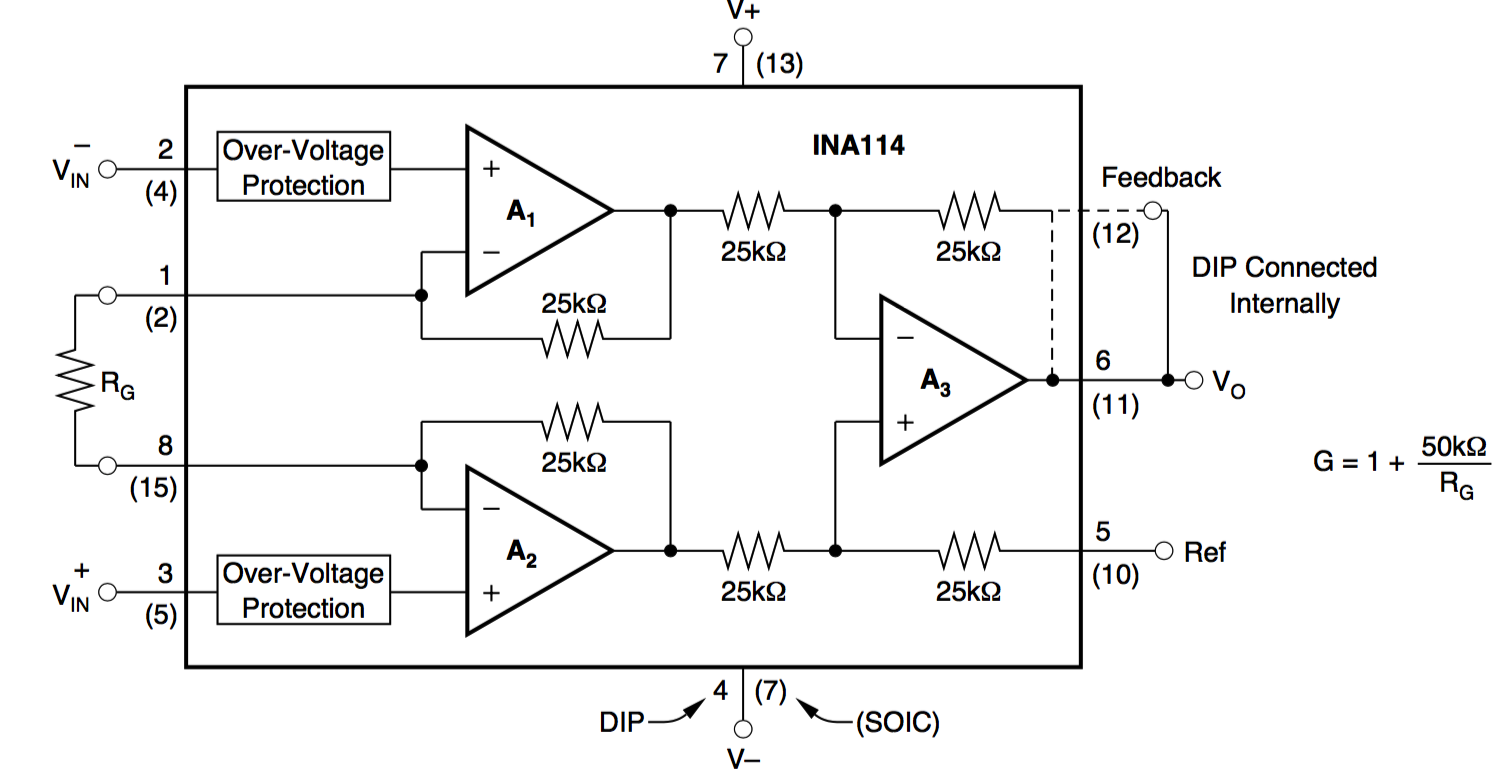
\includegraphics[width=1\textwidth]{Figurer/Snip20151117_104}
	\caption{INA114}
\end{figure}

INA114 er blevet udleveret som én komponent. Den sorte boks på Figur 3.1 viser, hvilke del-komponenter INA114 indeholder. Det ses også, at $R_{G}$ er placeret udenfor den sorte boks, hvilket betyder, at det er en variabel modstand, der skal tilkobles INA114.  
\\
\\
På Figur 3.2 ses, hvordan INA114 \footnote{Se datablad for INA114 i bilag} skal realiseres i forhold til at implementere forstærkeren. 

\begin{figure}[H]
	\centering
	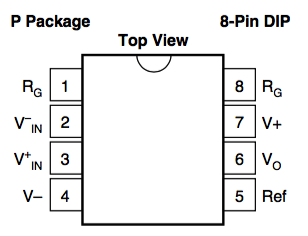
\includegraphics[width=0.6\textwidth]{Figurer/Snip20151207_47}
	\caption{INA114}
\end{figure}

På ben et og otte forbindes INA114 med gainmodstanden, $R_{G}$. Ben fire forbindes med -9 V. Ben syv forbindes med +9 V. Ben fem forbindes til jord. Indgangssignalet modtages ved ben to og tre, mens outputtet kommer fra ben seks, som forbindes med filteret, som viderebehandler signalet. 
   

\subsubsection{Forstærkning}
Forstærkningen, Gain, skal forstærke den maksimale inputsspænding fra tryktransduceren, så outputtet bliver 5 V, hvilket er det interval, der er valgt for DAQ'en. Udregningen for forstærkning kan ses i ligning (2.4) til (2.5).
\begin{equation}
	Gain = 666,667
\end{equation}


\subsubsection{Båndbredde}
For INA114 er produktet af båndbredden og forstærkningen en konstant på 1.000.000 \footnote{Se datablad for INA114 s. 2 i bilag}.
Båndbredden for denne forstærkerblok, hvor gain er 1333,33, er 

\begin{equation}
	Gain \cdot BW = 1.000.000 \\ \Longrightarrow \\
	BW = \frac{1.000.000}{666,667} \\ \Longrightarrow \\
	BW = 1500 Hz
\end{equation} 

Båndbredden er større end 50 Hz, som var det, båndbredden mindst skulle være. 

\subsubsection{Gainmodstand}
Gainmodstanden, $R_{G}$ er en variabel modstand, der bestemmer forstærkningen i INA114. INA114 skal have en gain på 666,667. Ud fra ligning (3.3) kan $R_{G}$ isoleres og beregnes.\\

\begin{equation}
	Gain = 1+\frac{50k\Omega}{R_g} \\ \Longrightarrow \\
	R_{G} = \frac{50k\Omega}{Gain - 1} \\ \Longrightarrow \\
	R_{G} = \frac{50k\Omega}{666,667 - 1} \\ \Longrightarrow \\
	R_{G} = 75\Omega
\end{equation}


\subsection{Filterblok}
Som filter anvendes et Sallen Key lavpasfilter med unity gain.

\begin{figure}[H]
	\centering
	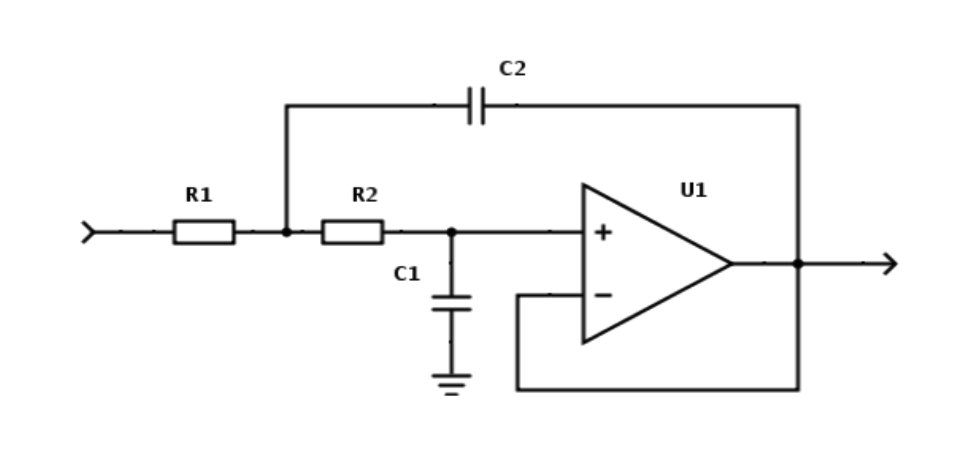
\includegraphics[width=1\textwidth]{Figurer/Snip20151117_105}
	\caption{Sallen Key lavpasfilter}
\end{figure}

Som ikke-inverterende operationsforstærker anvendes der OP27G \footnote{Se datablad for OP27G i bilag}, se Figur 3.4. 

\begin{figure}[H]
	\centering
	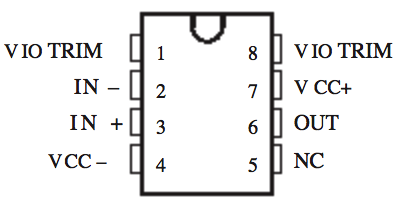
\includegraphics[width=0.5\textwidth]{Figurer/Snip20151207_49}
	\caption{OP27G}
\end{figure}

Ben tre modtager det forstærket signal. Ben to forbindes med ben seks, hvor det færdig behandlede signal kan måles. Ben fire forbindes med -9 V. Ben syv forbindes med +9 V.  


\subsubsection{Beregning af komponentværdier}
Ud fra overføringsfunktion for filteret kan de forskellige komponentværdier beregnes. 

\subsubsection{Overføringsfunktion}
\begin{align}
	\frac{V_{out}(s)}{V_{in}(s)}=\frac{\frac{1}{R_1R_2C_1C_2}}{s^2+\frac{R_1+R_2}{R_1R_2C_2}+\frac{1}{R_1R_2C_1C_2}}
\end{align}

\subsubsection{Standardform}
\begin{align}
	\frac{V_{out}(s)}{V_{in}(s)}=\frac{w_n^2}{s^2+2\zeta\omega _n+w_n^2}
\end{align}

\begin{align}
	\omega _n = \sqrt{\frac{1}{R_1R_2C_1C_2}}
\end{align}

Kondensatoren, C2, skal være 680 nF og kondensatoren, C1, bestemmes til 340 nF, da denne kondensator kunne realiseres ud fra det, der var til rådighed. Der benyttes en kondensator på 330 nF og 10 nF til den realisering. Modstandene R1 og R2 skal være samme værdi, R = R1 = R2    

\begin{equation}
	50*2\pi = \sqrt{\frac{1}{R*340*10^{-9}*680*10^{-9}}} \\ \Longrightarrow \\
	Solve, R \\ \Longrightarrow \\
	R = 6620 \Omega
\end{equation}

Ved realiseringen af de to modstande vælge 3k$\Omega$ og 3.6k$\Omega$.  

\subsubsection{Magnitude Bodeplot}
Bodeplottet i Figur 3.3 viser, at ved -3 dB, hvor cutofffrekvens befinder sig er frekvensen 50 Hz, som var et krav. Det ses også, at grafen er faldet med 40 dB en dekade efter, 500 Hz, som også var et krav.   
\begin{figure}[H]
	\centering
	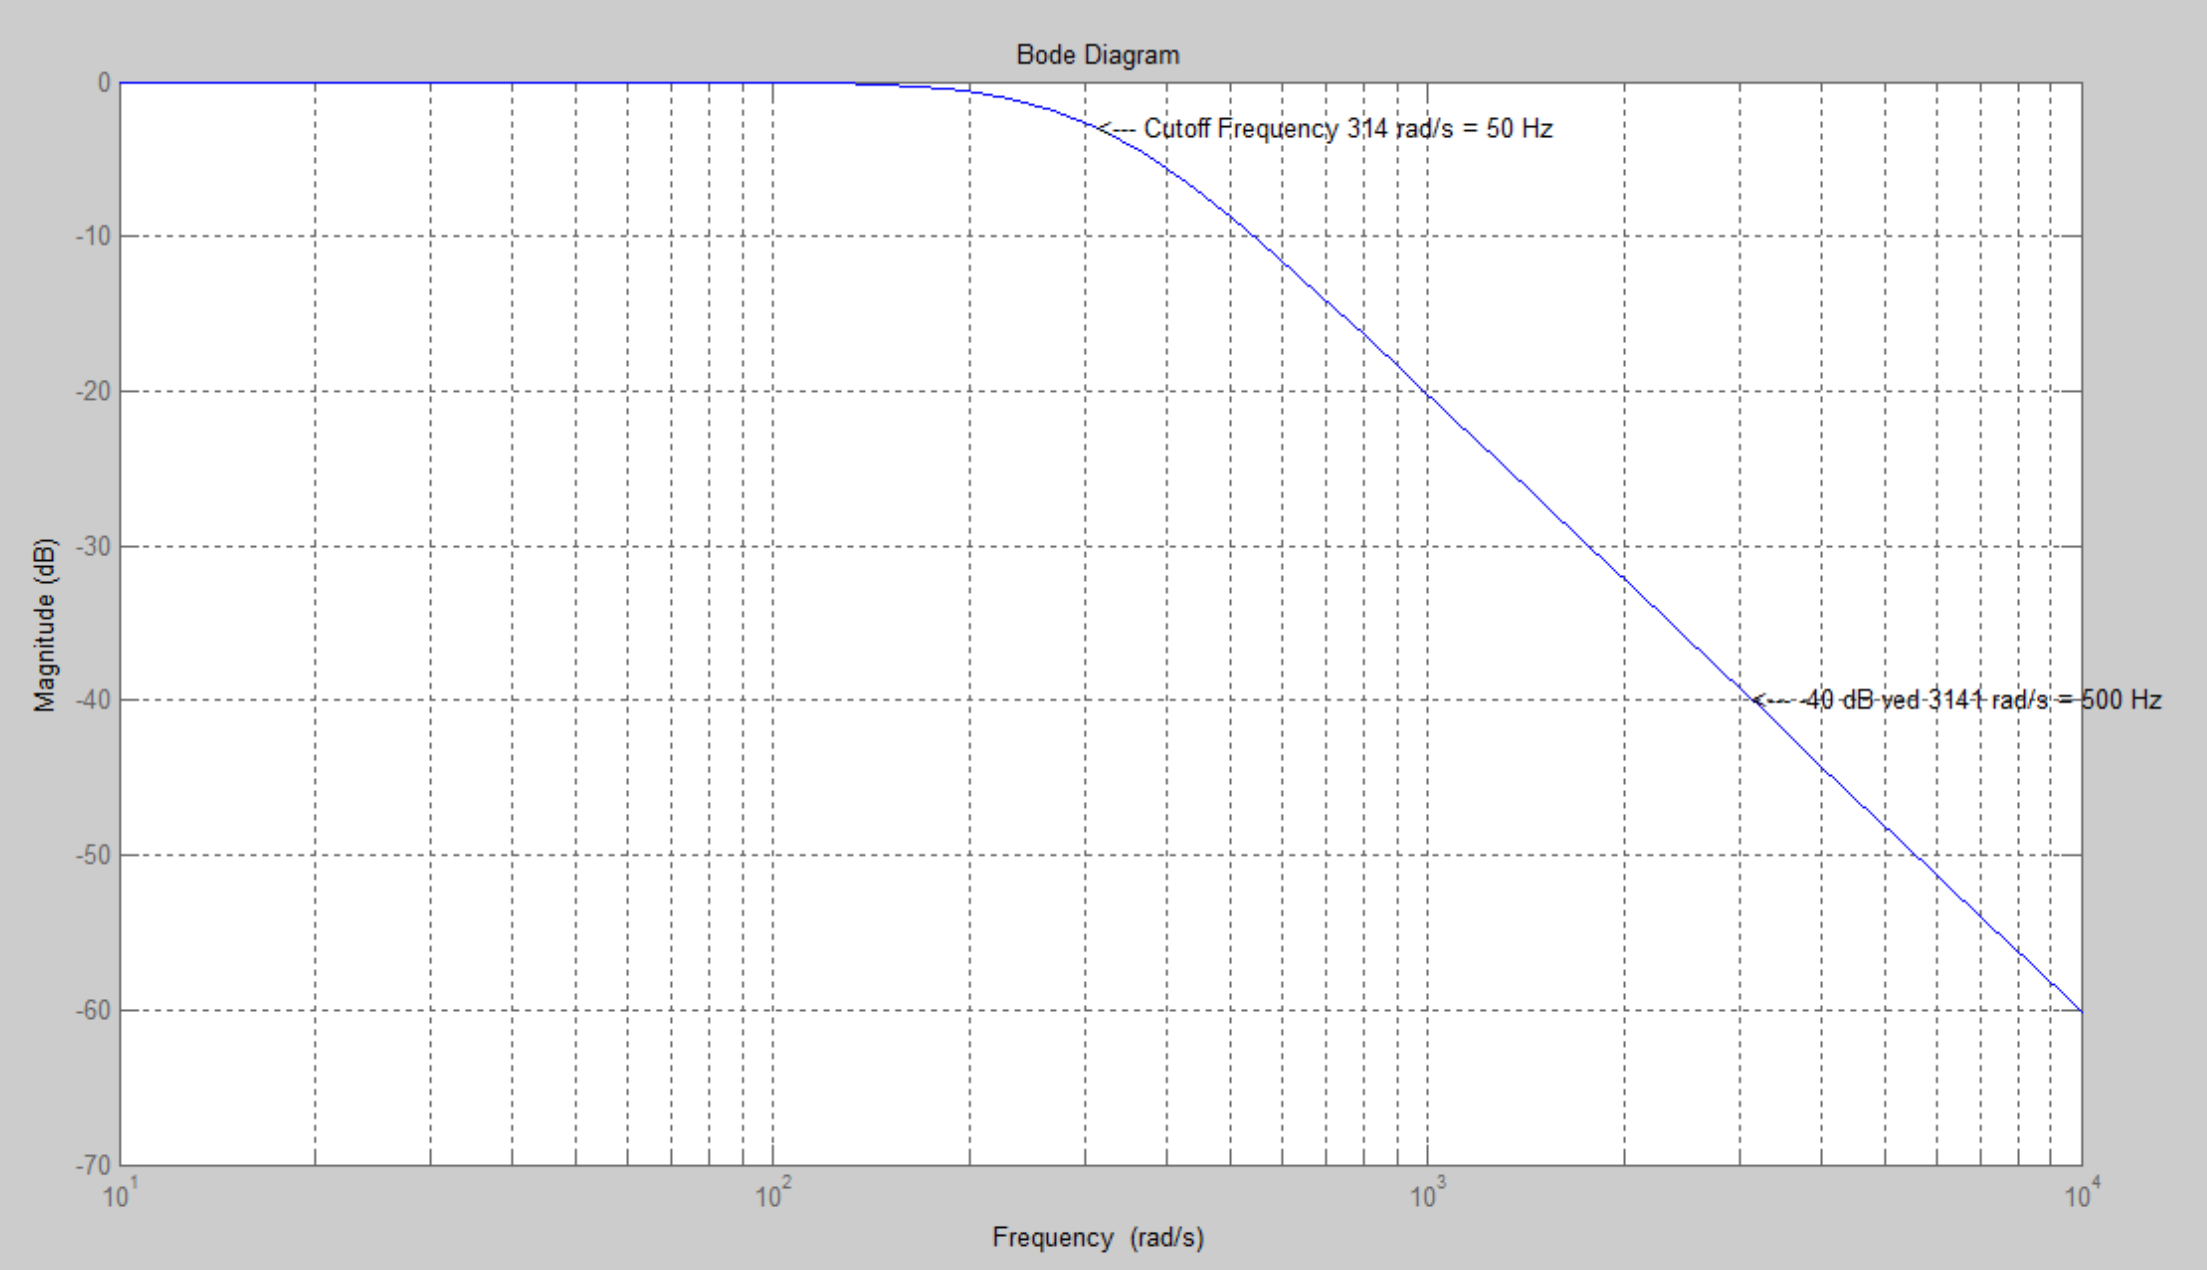
\includegraphics[width=1\textwidth]{Figurer/Bodeplot_Lavpasfilter_Teoretisk}
	\caption{Magnitude Bodeplot Lavpasfilter}
	\label{fig:Bodeplot}
\end{figure}

\section{Test}
Forstærkeren og filteret testes via Analog Discovery \& Waveforms. De testes både hver for sig og sidst sammen som signalbehandlingsblok.\\ 

\subsection{Test af forstærkerblok}
Testopstillingen kan ses på Figur 3.4. 

\begin{figure}[H]
	\centering
	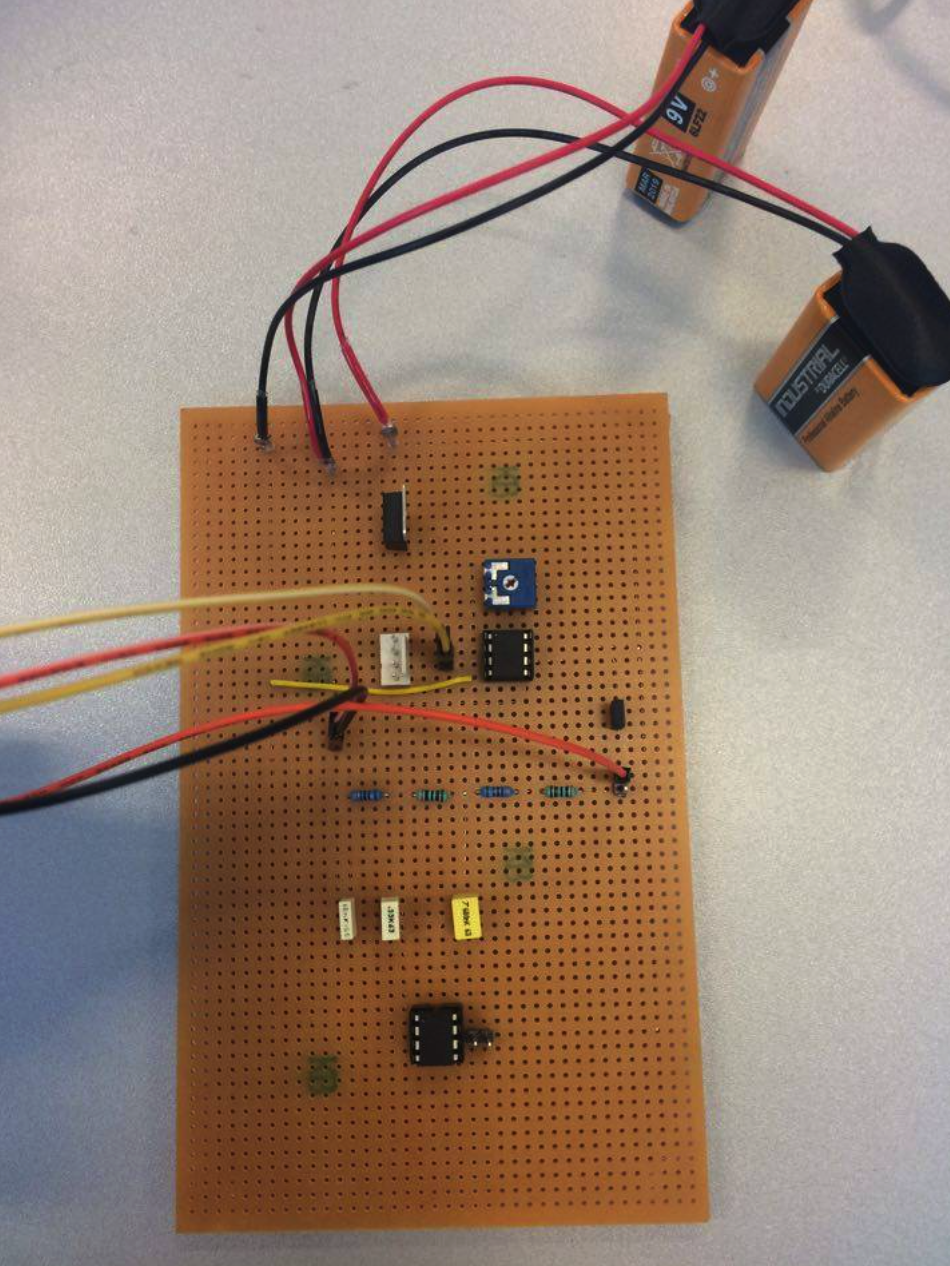
\includegraphics[width=0.8\textwidth]{Figurer/Snip20151207_35}
	\caption{Testopstilling for forstærkeren}
\end{figure}

Der ønskes, at ved en indgangsspænding på 7,5 mV vil outputsspændingen være forstærket op til 5 V. Der kunne ikke påtrykkes en spænding på 7,5 mV, men istedet med 7 mV. Outputsspændingen ved 7 mV er 

\begin{equation}
	7 mV \cdot 666,667 = 4,7 V
\end{equation} 

Dette ser, at være det samme, når man tester forstærkeren, se figur 3.5. 

\begin{figure}[H]
	\centering
	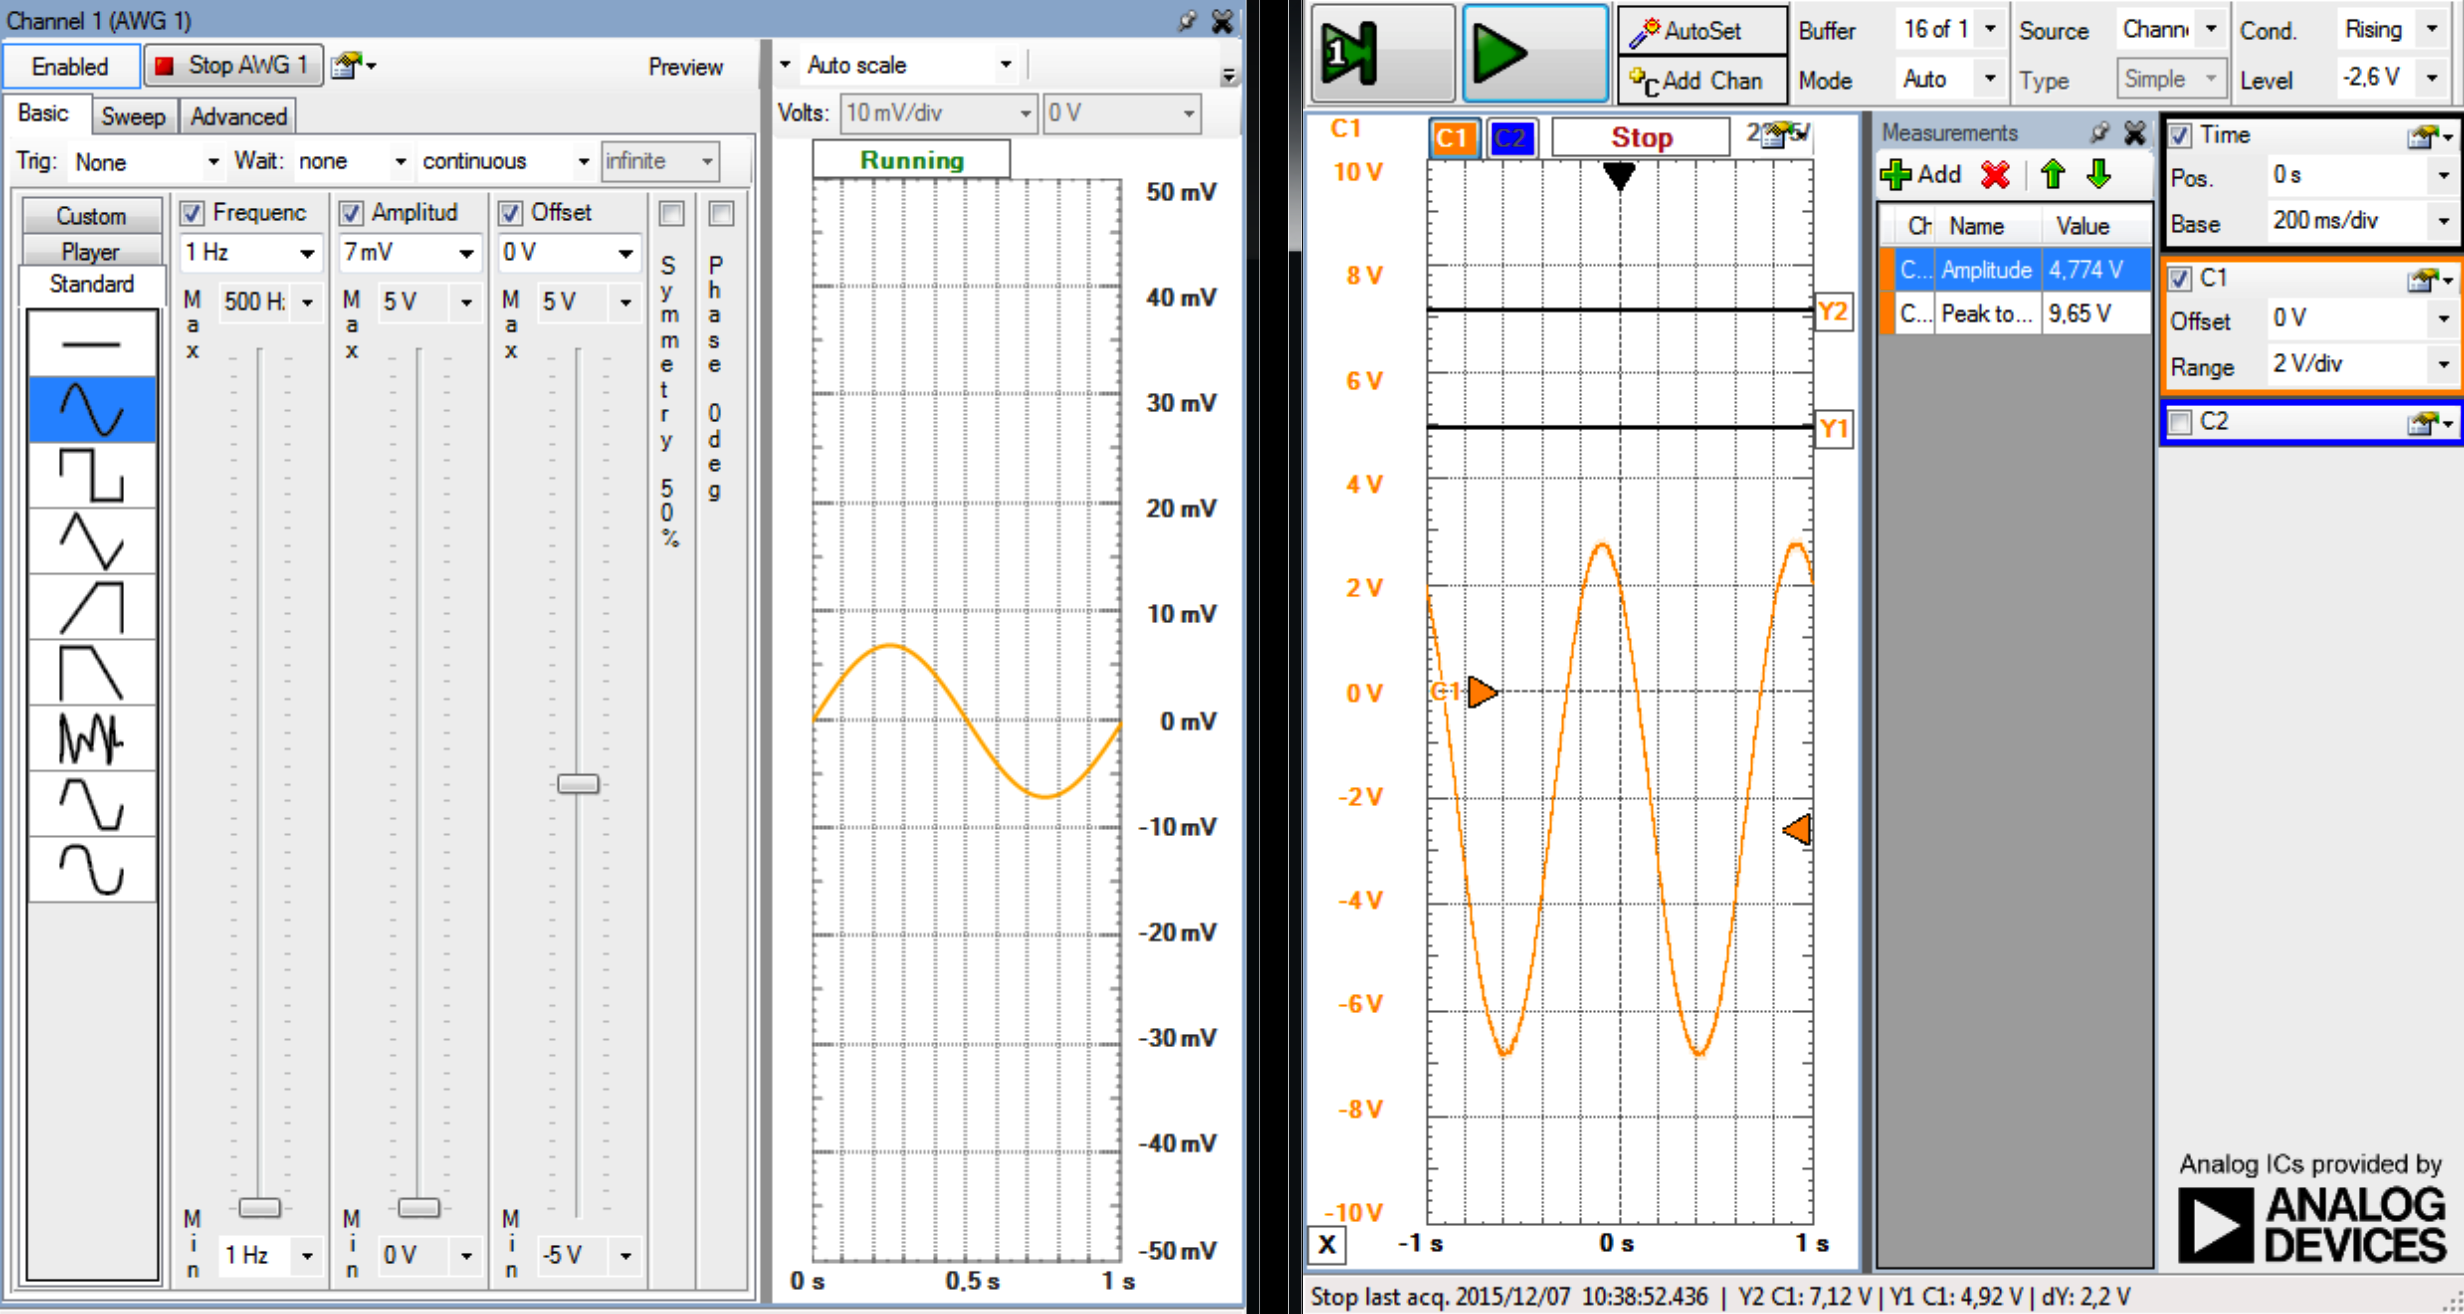
\includegraphics[width=1\textwidth]{Figurer/Snip20151207_37}
	\caption{Forstærker respons ved 7 mV}
\end{figure}


\subsection{Test af filterblok}
Testen af filteret foretaget, hvor der påtrykkes en AC spænding på 5 V, hvor frekvensen varieres imellem 1 Hz, 50 Hz og 500 Hz. \\ \\

Testopstillingen ses på Figur 3.6.  

\begin{figure}[H]
	\centering
	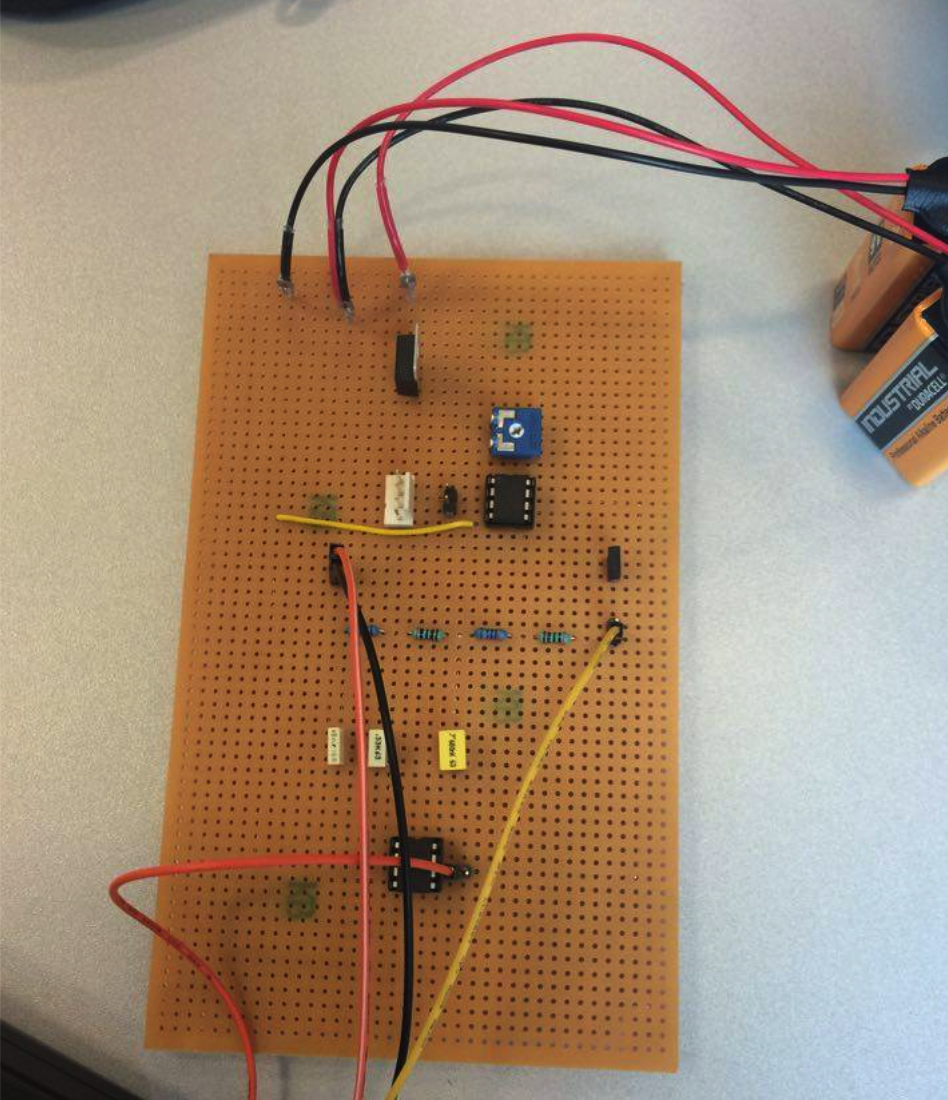
\includegraphics[width=0.8\textwidth]{Figurer/Snip20151207_38}
	\caption{Testopstilling af filteret}
	\label{fig:Filter}
\end{figure}

Channel 1 er indgangsspændingen og viser den varierende frekvens. Ændringen ses i venstre side af efterfølgende skærmbilleder. 
Oscilloskopet måler udgangsspændingen på filteret og resultatet vises i højre side af efterfølgende skærmbilleder.

\subsubsection{Filtering ved 1 Hz}
\begin{figure}[H]
	\centering
	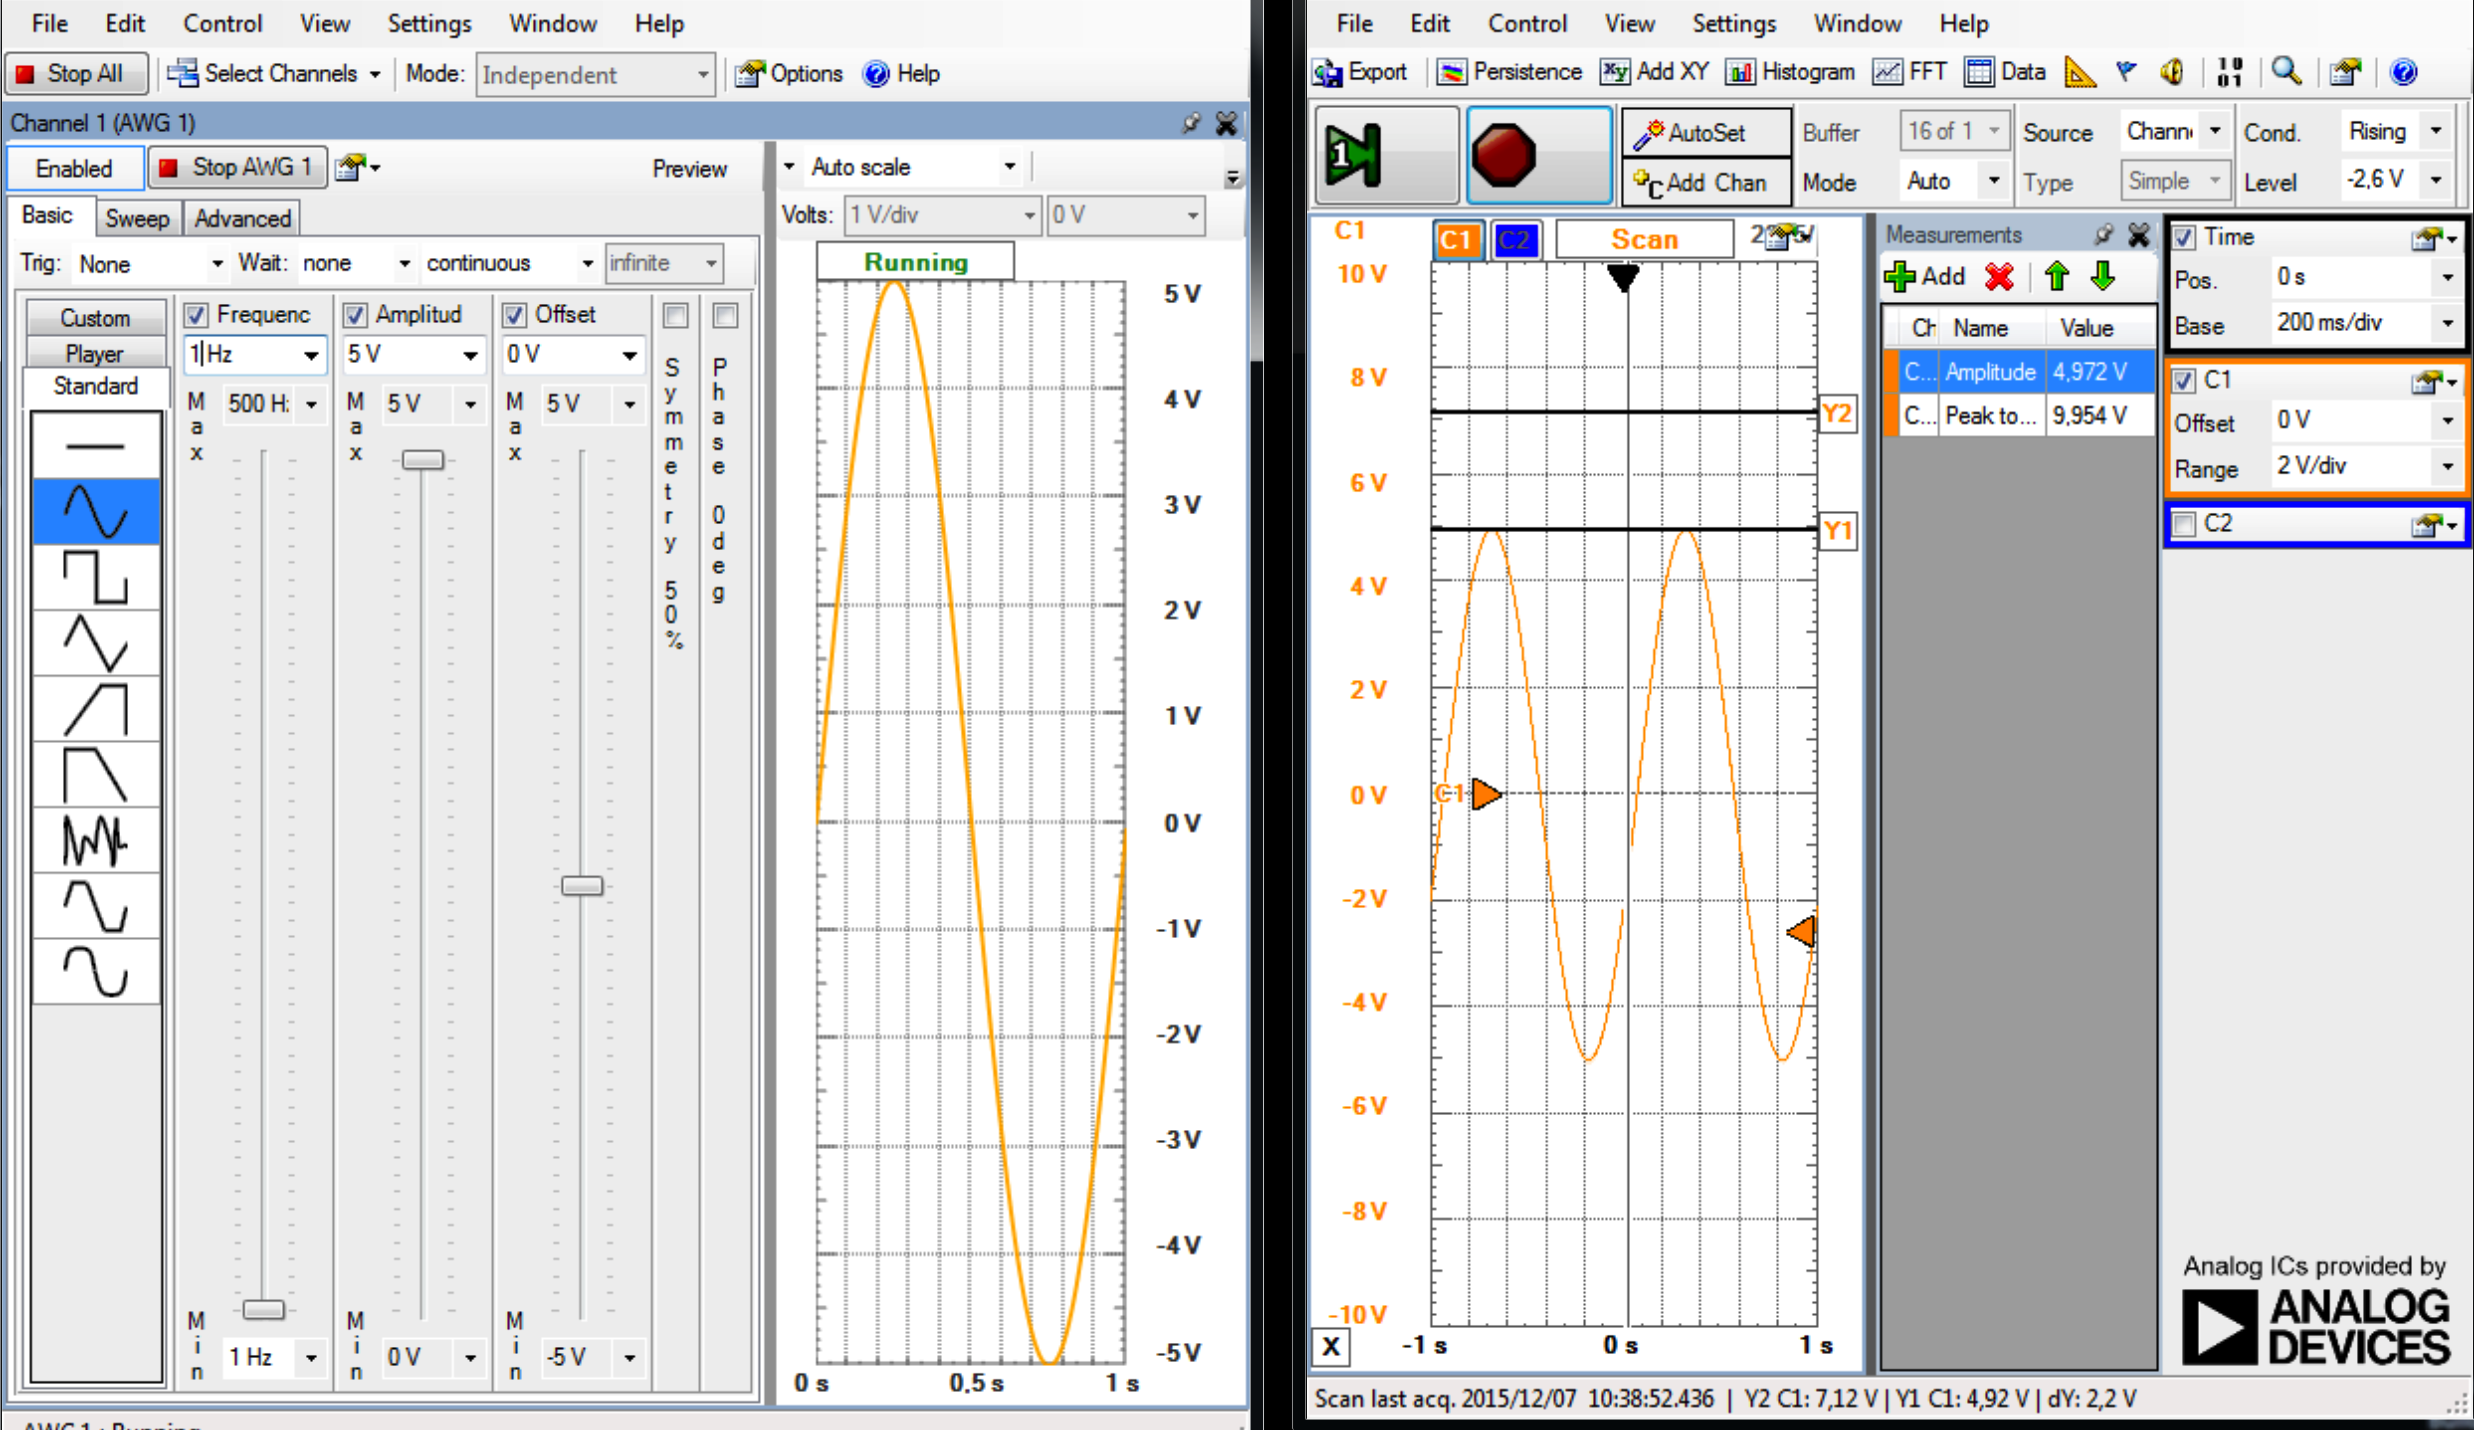
\includegraphics[width=1\textwidth]{Figurer/Snip20151207_39}
	\caption{Lavpasfilter respons 1 Hz}
	\label{fig:Filter}
\end{figure}

På figur 3.7 ses det, at indgangsspændingen  og outputspændingen er den samme - 5 V ca. Dette er også det ønskede resultat, da filteret er et lavpasfilter, der er designet til at lukke de lave frekvenser igennem indtil 50 Hz. 
 
\subsubsection{Filtering ved 50 Hz}
\begin{figure}[H]
	\centering
	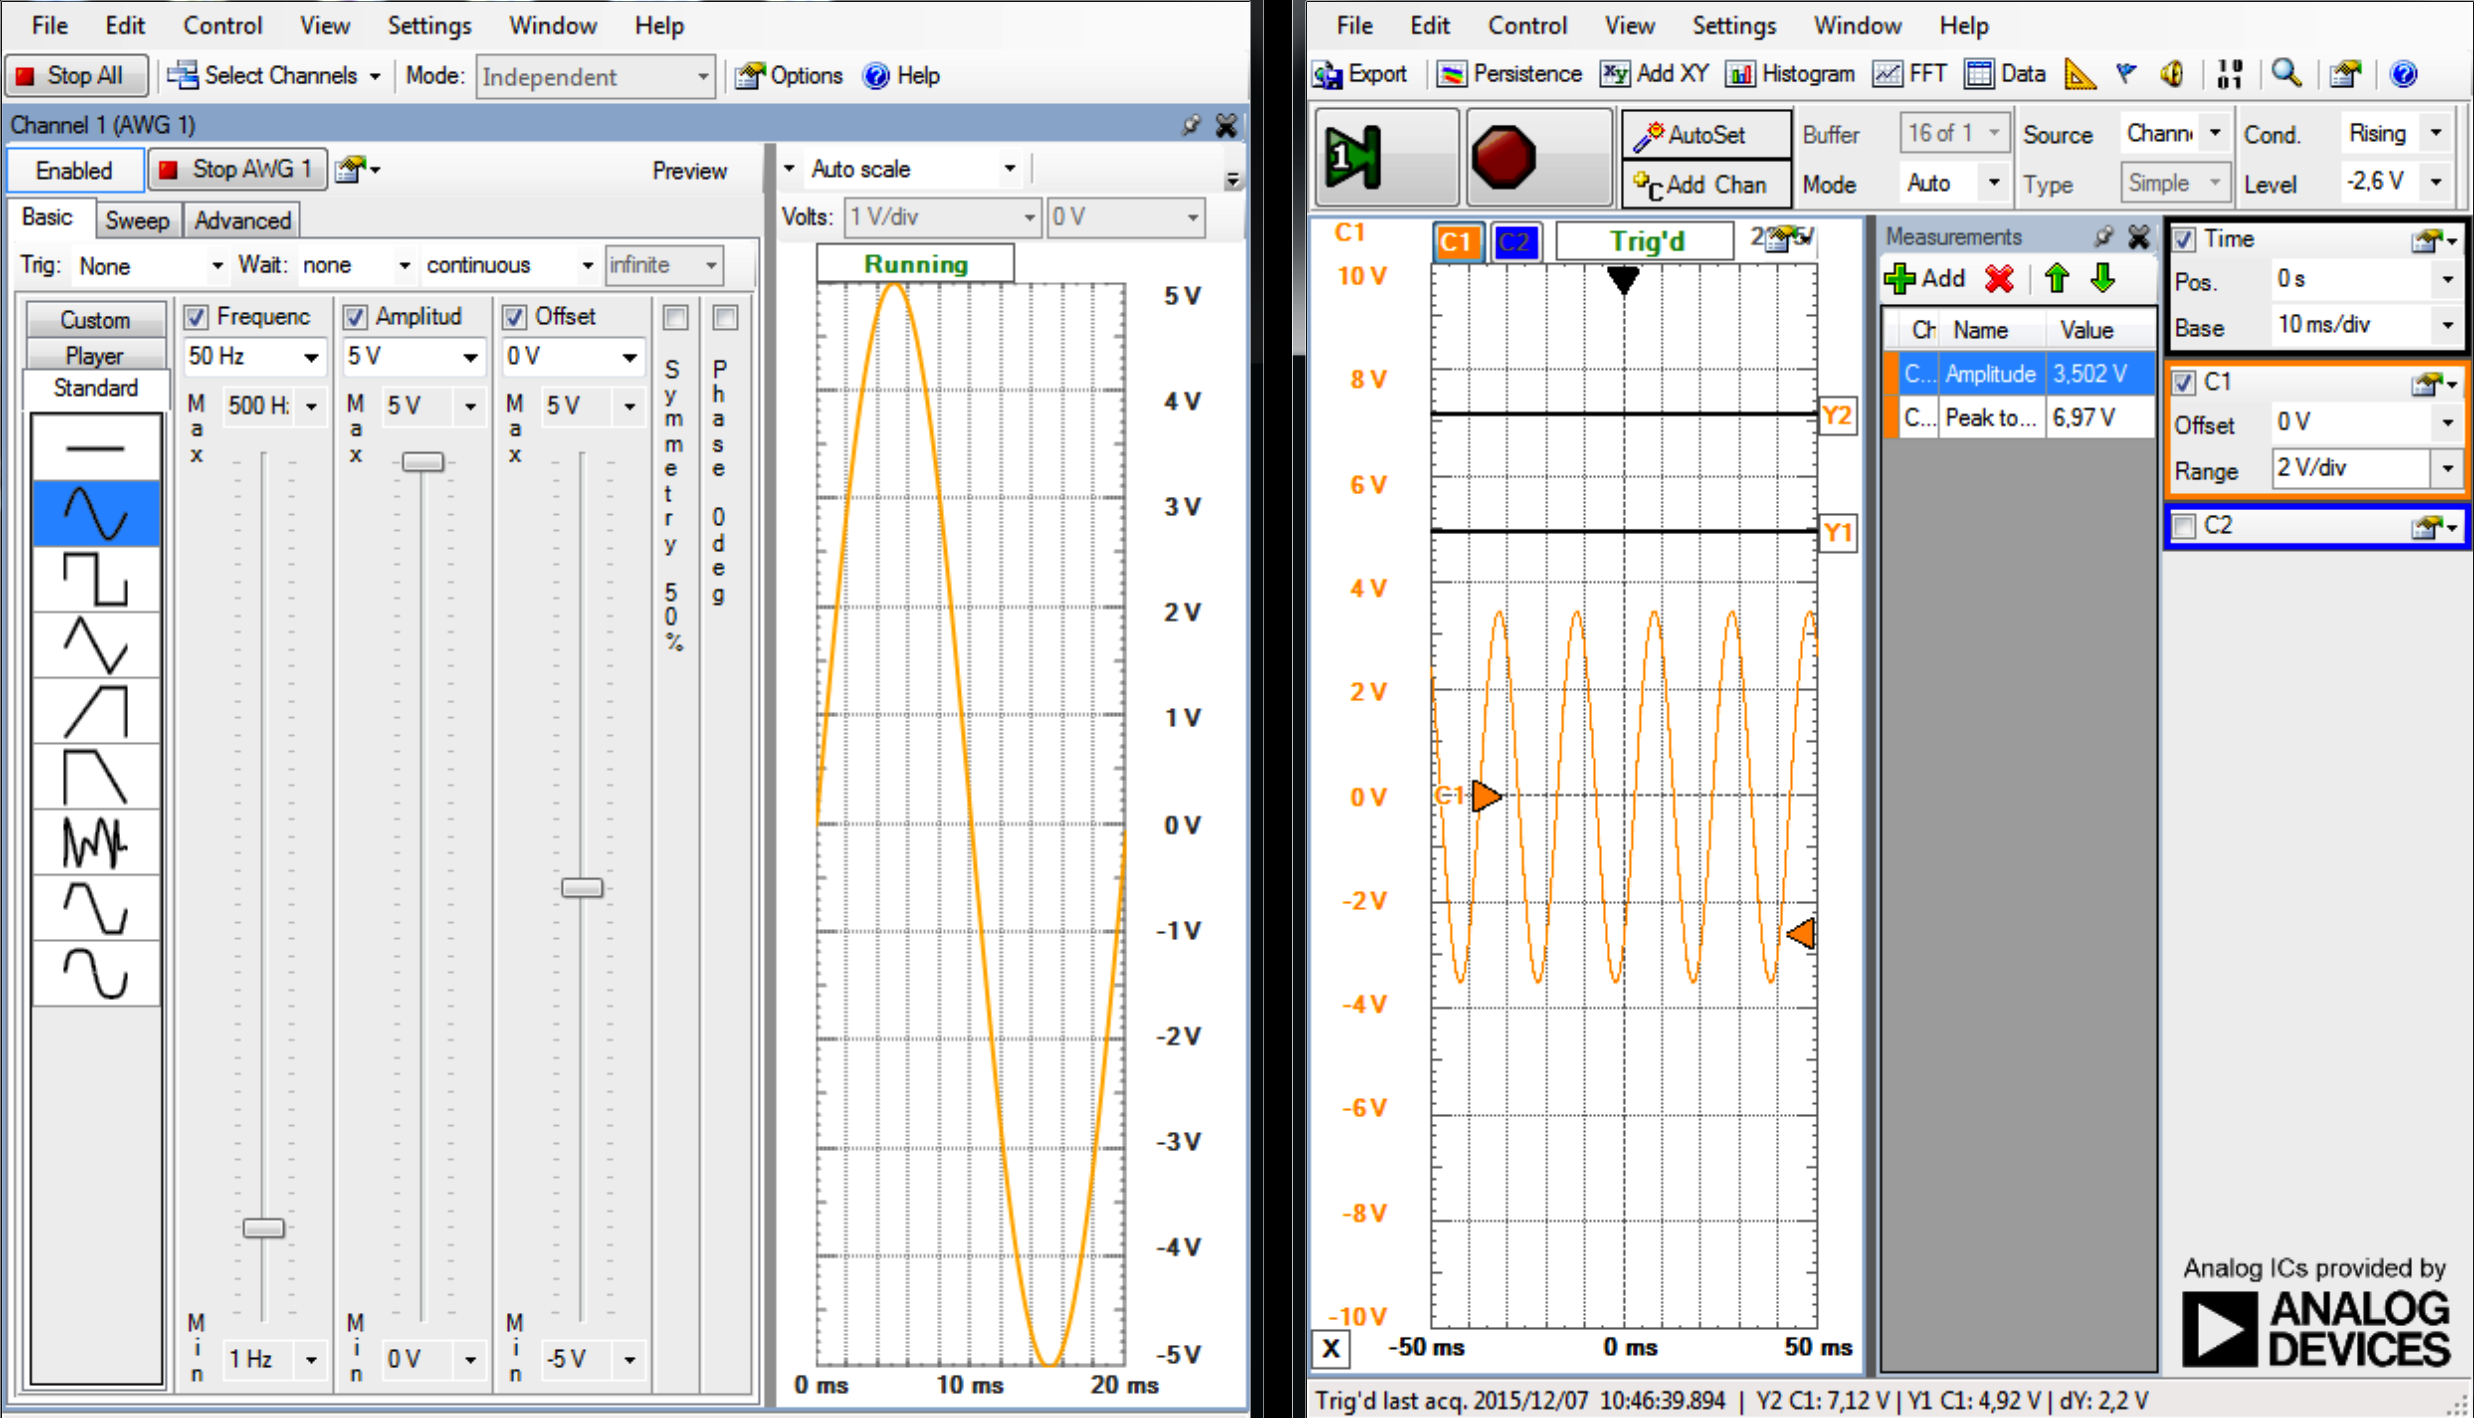
\includegraphics[width=1\textwidth]{Figurer/Snip20151207_40}
	\caption{Lavpasfilter respons 50 Hz}
	\label{fig:Filter}
\end{figure}

Ved 50 Hz, som er filteret cutofffrekvens, skal indgangsspændingen være dæmpet med 3 dB efter filteringen. I ligningen (3.9) beregnes, hvad outputspændingen er efter en dæmpning med 3 dB. 

\begin{equation}
	3 dB = 20\cdot log(x) \\ \Longrightarrow \\
	x = 0,707 \\ \Longrightarrow \\
	outputspænding = 5 V \cdot 0,707 \\ \Longrightarrow \\
	outputspænding = 3,535 V 
\end{equation}

På Figur 3.8 ses, at det i praksis er 3,502 V, hvilket der er acceptabelt. 

\subsubsection{Filtering ved 500 Hz}

\begin{figure}[H]
	\centering
	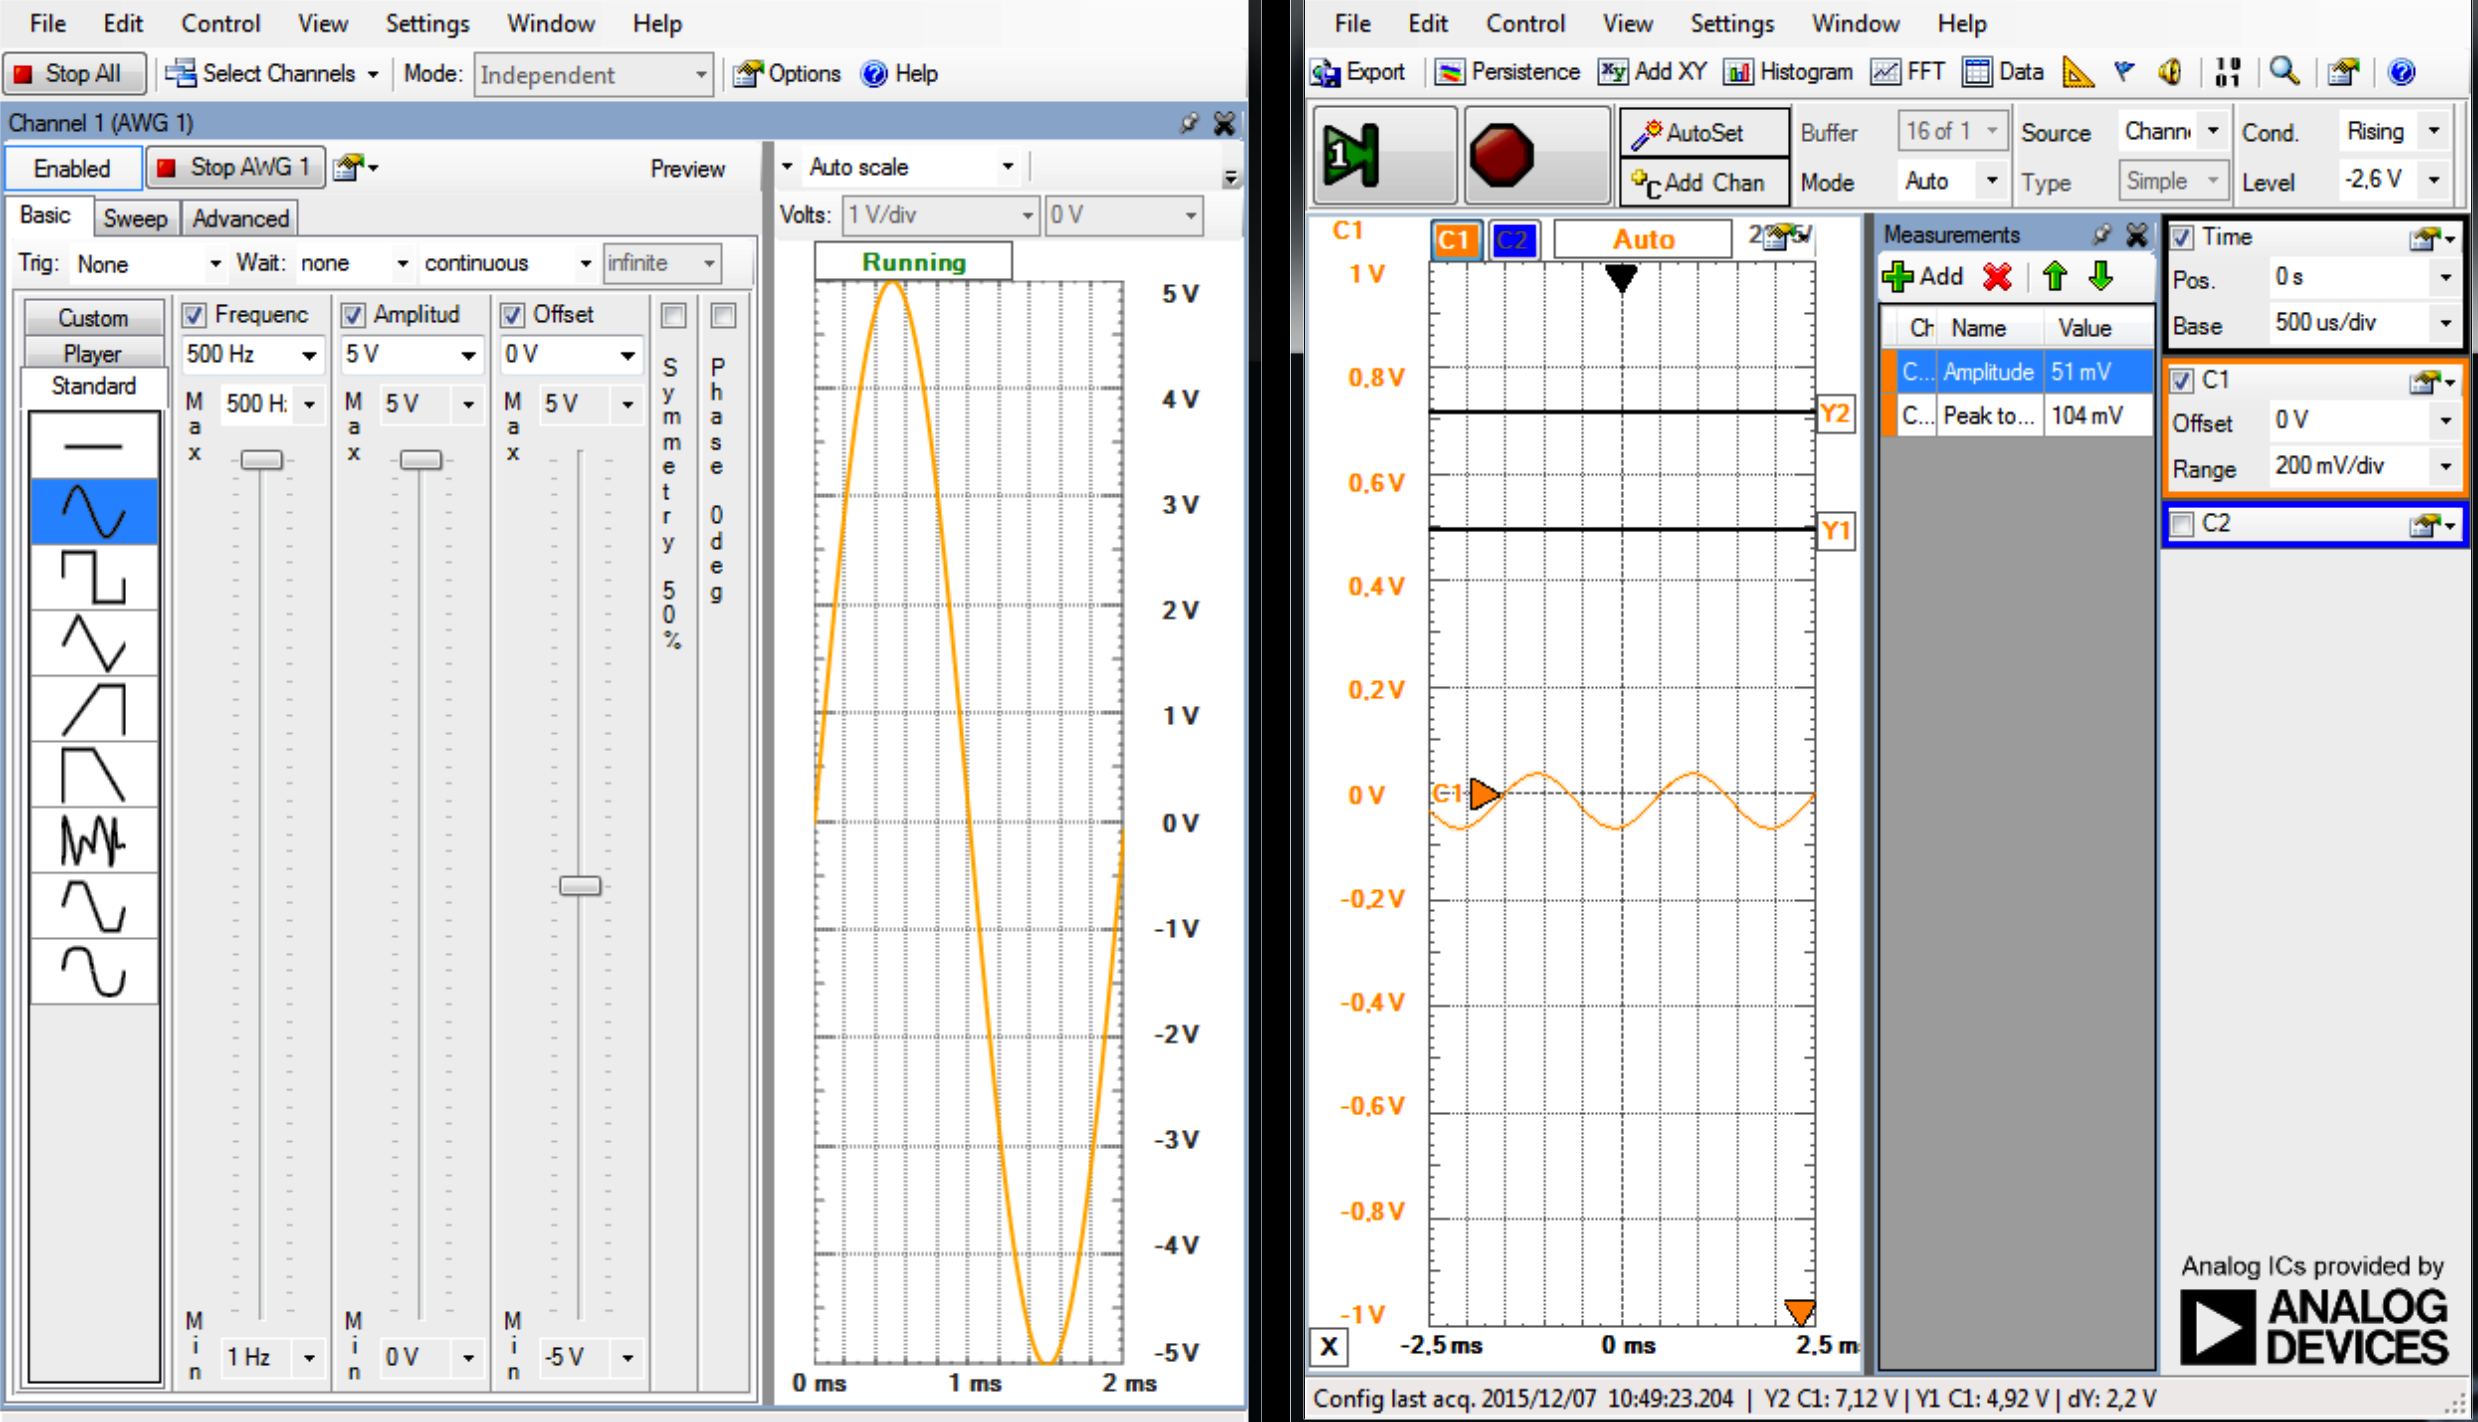
\includegraphics[width=1\textwidth]{Figurer/Snip20151207_41}
	\caption{Lavpasfilter respons 500 Hz}
	\label{fig:Filter}
\end{figure}

Her forventes, der en dæmpning med 40 dB, da det er et andenordens lavpasfilter, og 500 Hz er en dekade efter cutofffrekvensen. I ligning (3.10) ses beregningen, hvad outputspændingen er efter en dæmpning på 40 dB. 

\begin{equation}
	40 dB = 20\cdot log(x) \\ \Longrightarrow \\
	x = 0,01 \\ \Longrightarrow \\
	outputspænding = 5 V \cdot 0,01  \\ \Longrightarrow \\
	outputspænding = 0,05 V 
\end{equation}

På Figur 3.9 ses, at det i praksis er 51 mV. Det omregnes til 0,051 V, hvilket er acceptabelt i forhold til teorien. 

\subsection{Test af signalbehandlingblok}

Testopstillingen ses på Figur 3.10. 

\begin{figure}[H]
	\centering
	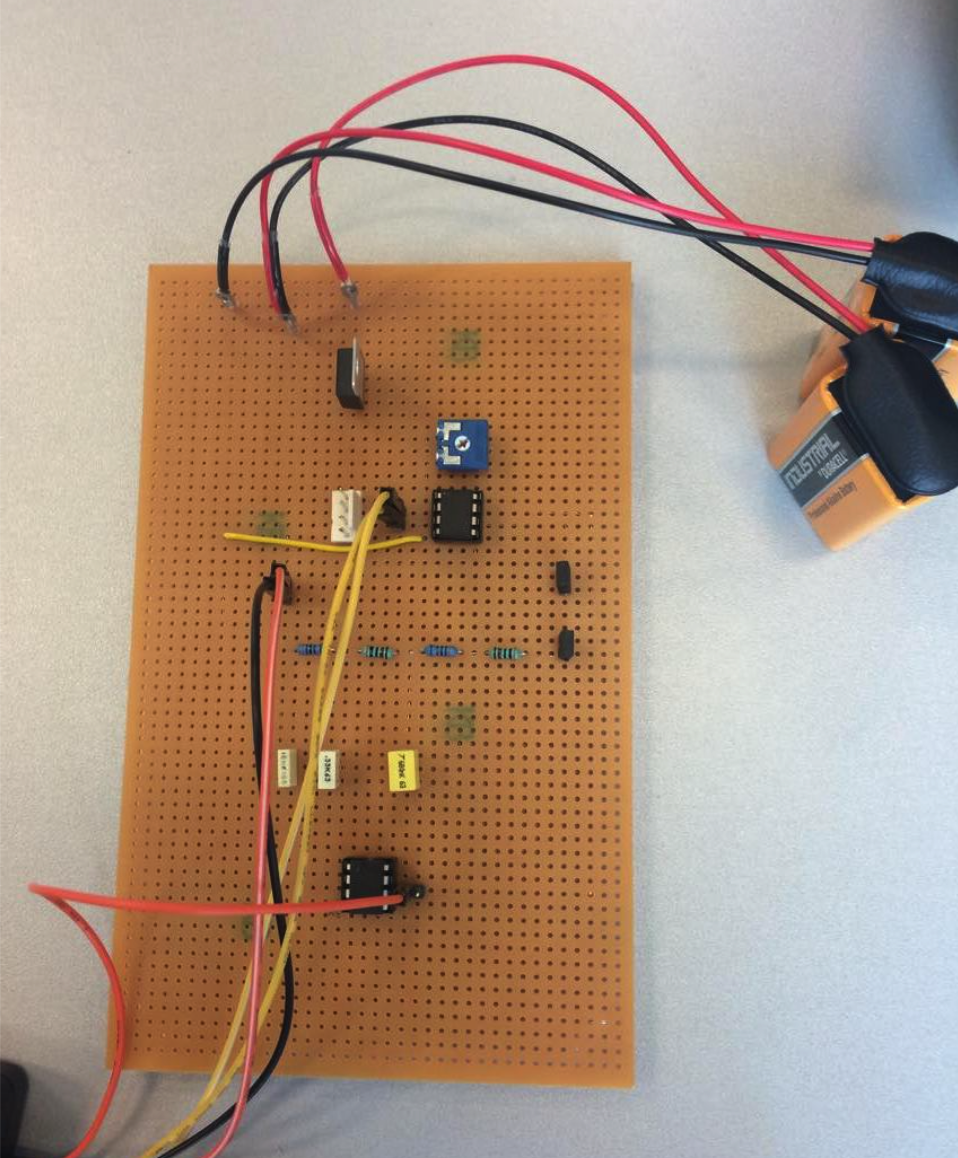
\includegraphics[width=0.8\textwidth]{Figurer/Snip20151207_46}
	\caption{Testopstilling af signalbehandlingblok}
	\label{fig:Signalbehanlding}
\end{figure}

Der laves tre forskellige tests, hvor frekvensen varieres mellem 1 Hz, 50 Hz og 500 Hz. Indgangsspændingen er i alle tests 13 mV. 
\\
\subsubsection{Test ved 1 Hz}
På Figur 3.11 ses resultatet ved 1 Hz. Der forventes, at forstærkeren har forstærket signalet op til 5 V samt at filteret ikke har påvirket outputtet, da frekvensen er under 50 Hz, som er filteret cutoffrekvens.
\\ \\
I praksis er det lig med 4,83 V - hvilket er acceptabelt.  
 
\begin{figure}[H]
	\centering
	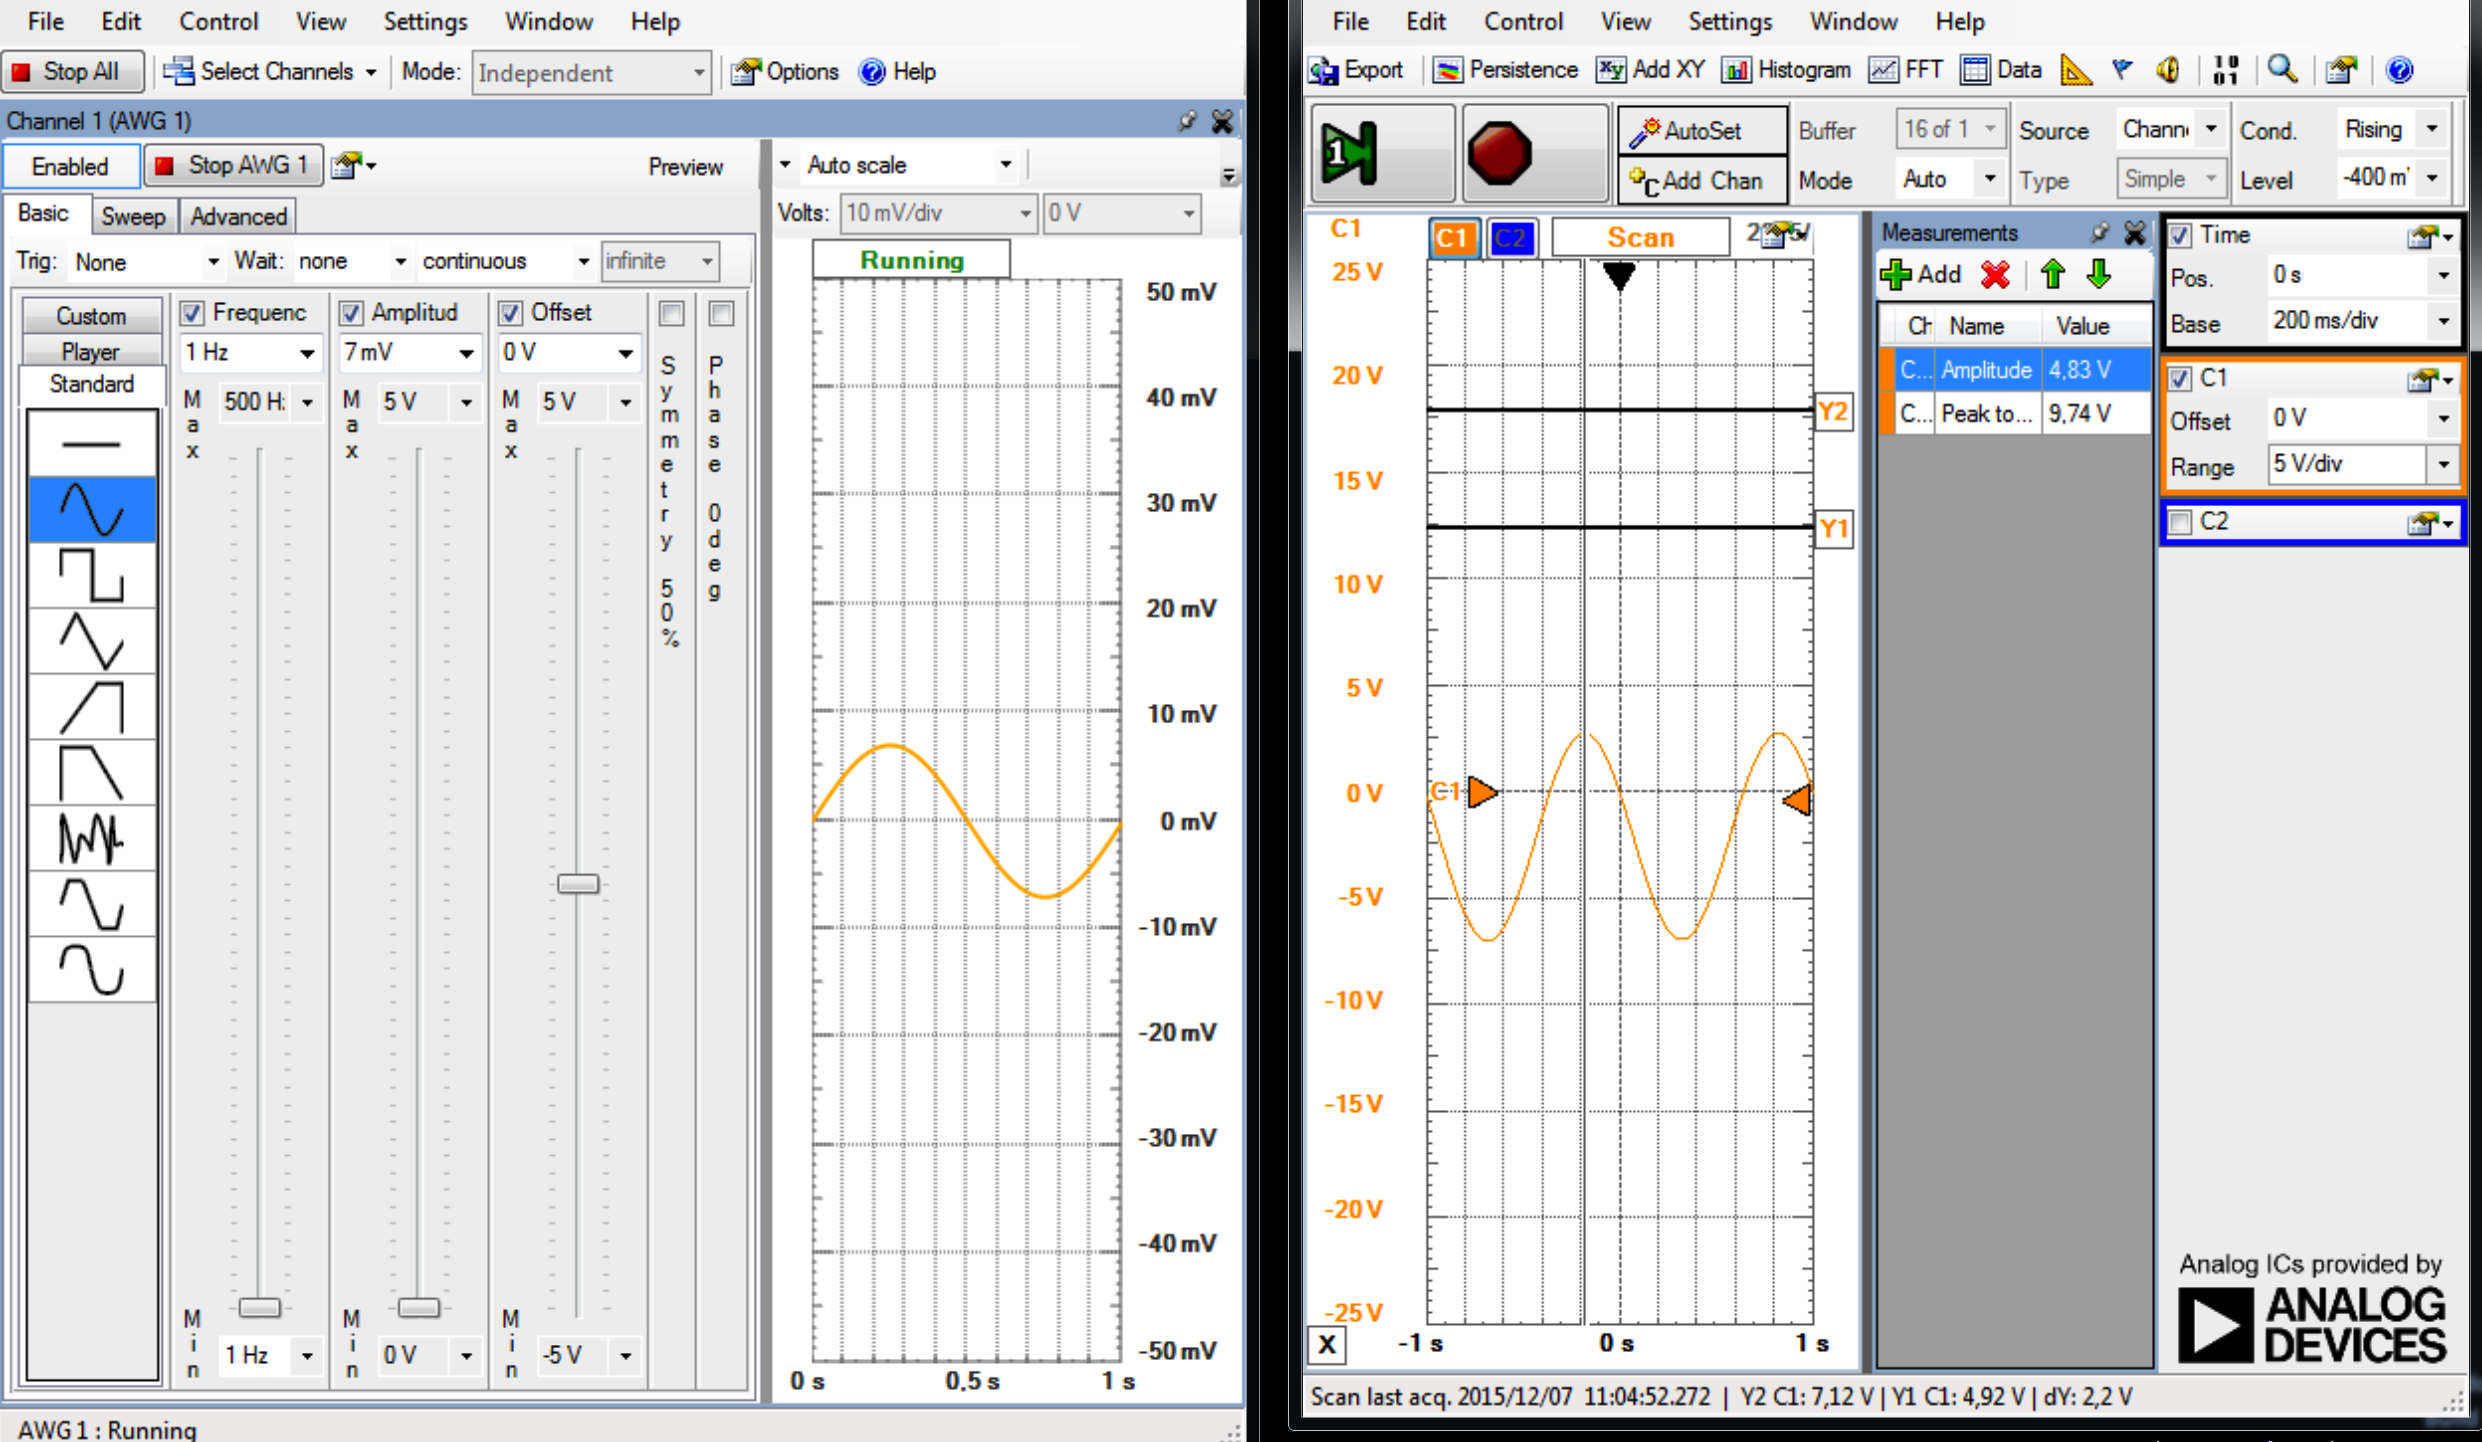
\includegraphics[width=1\textwidth]{Figurer/Snip20151207_42}	\caption{Signalbehanlding respons 1 Hz}
	\label{fig:Signalbehanlding}
\end{figure}

\subsubsection{Test ved 50 Hz}
På Figur 3.12 ses resultatet ved 50 Hz. Der forventes, at forstærkeren har forstærket signalet op til 5 V samt at filteret har dæmpet outputspændingen med 3 dB, så outputspændingen er lig med 3,535 V. 
\\ \\
I praksis er det lig med 3,39 V - hvilket er acceptabelt.    
  

\begin{figure}[H]
	\centering
	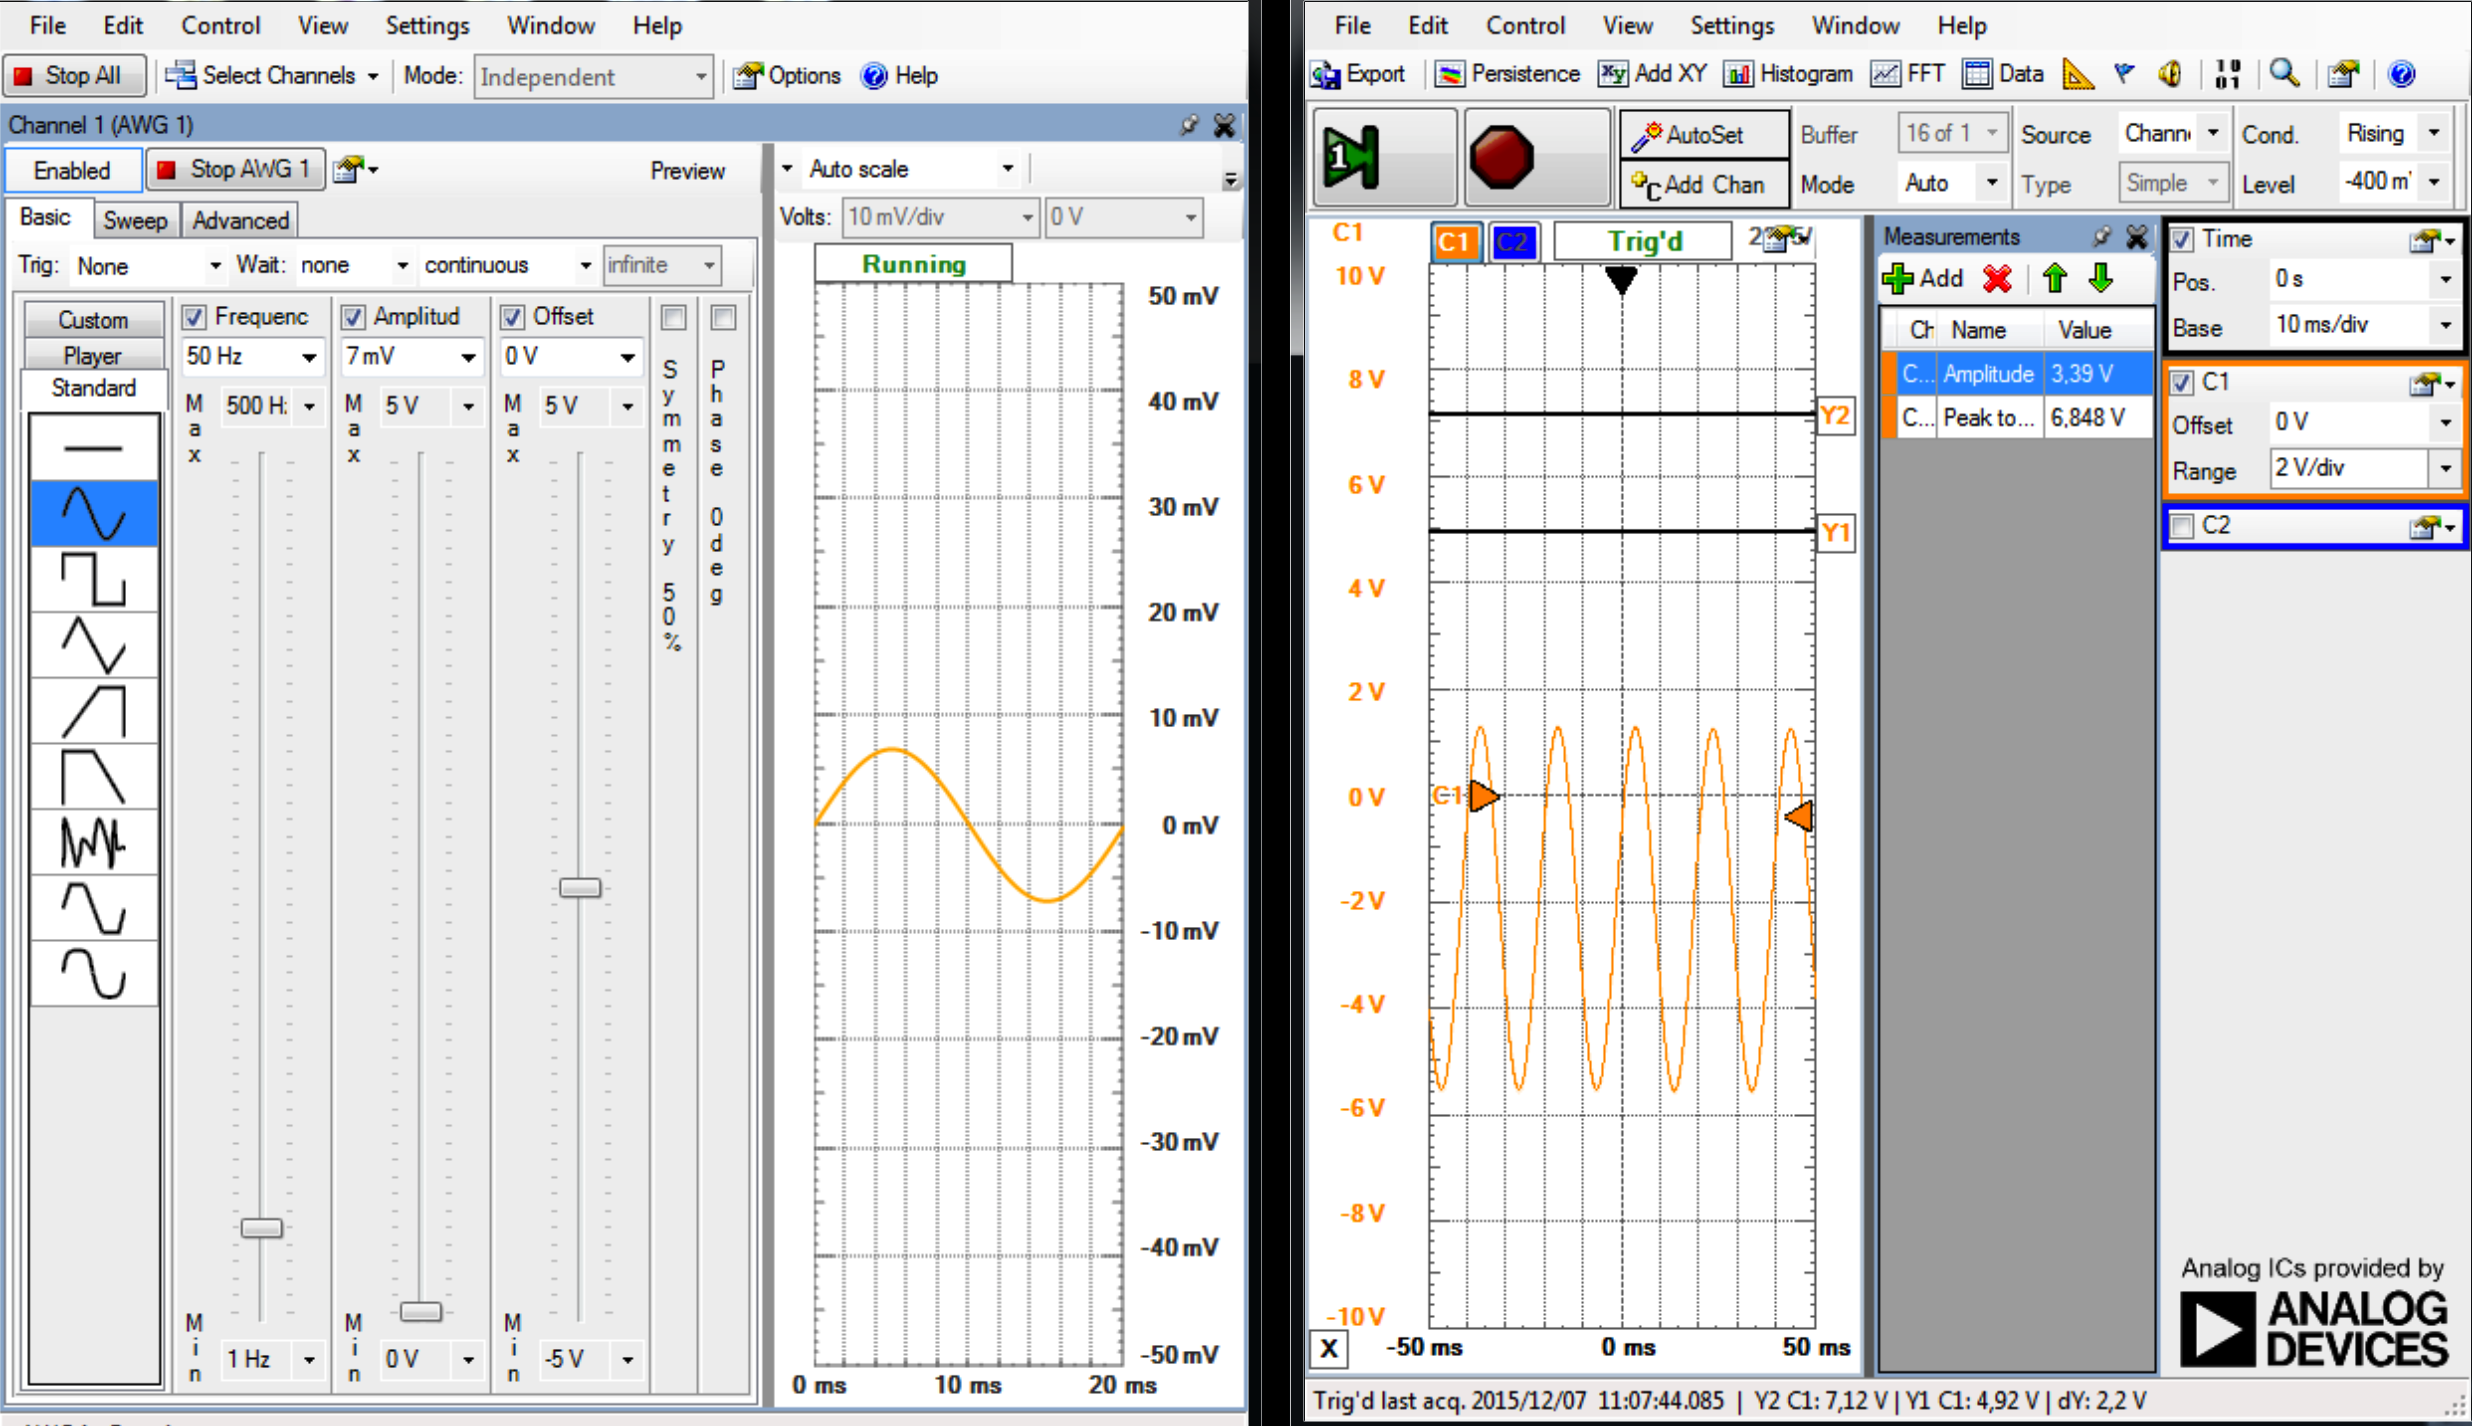
\includegraphics[width=1\textwidth]{Figurer/Snip20151207_43}
	\caption{Signalbehanlding respons 50 Hz}
	\label{fig:Signalbehanlding}
\end{figure}

\subsubsection{Test ved 500 Hz}
På Figur 3.13 ses resultatet ved 500 Hz. Der forventes, at forstærkeren har forstærket signalet op til 5 V samt at filteret har dæmpet outputspændingen med 40 dB, så outputspændingen er lig med 0,05 V.    
\\ \\
I praksis er det lig med 0,056 V - hvilket er acceptabelt. 

\begin{figure}[H]
	\centering
	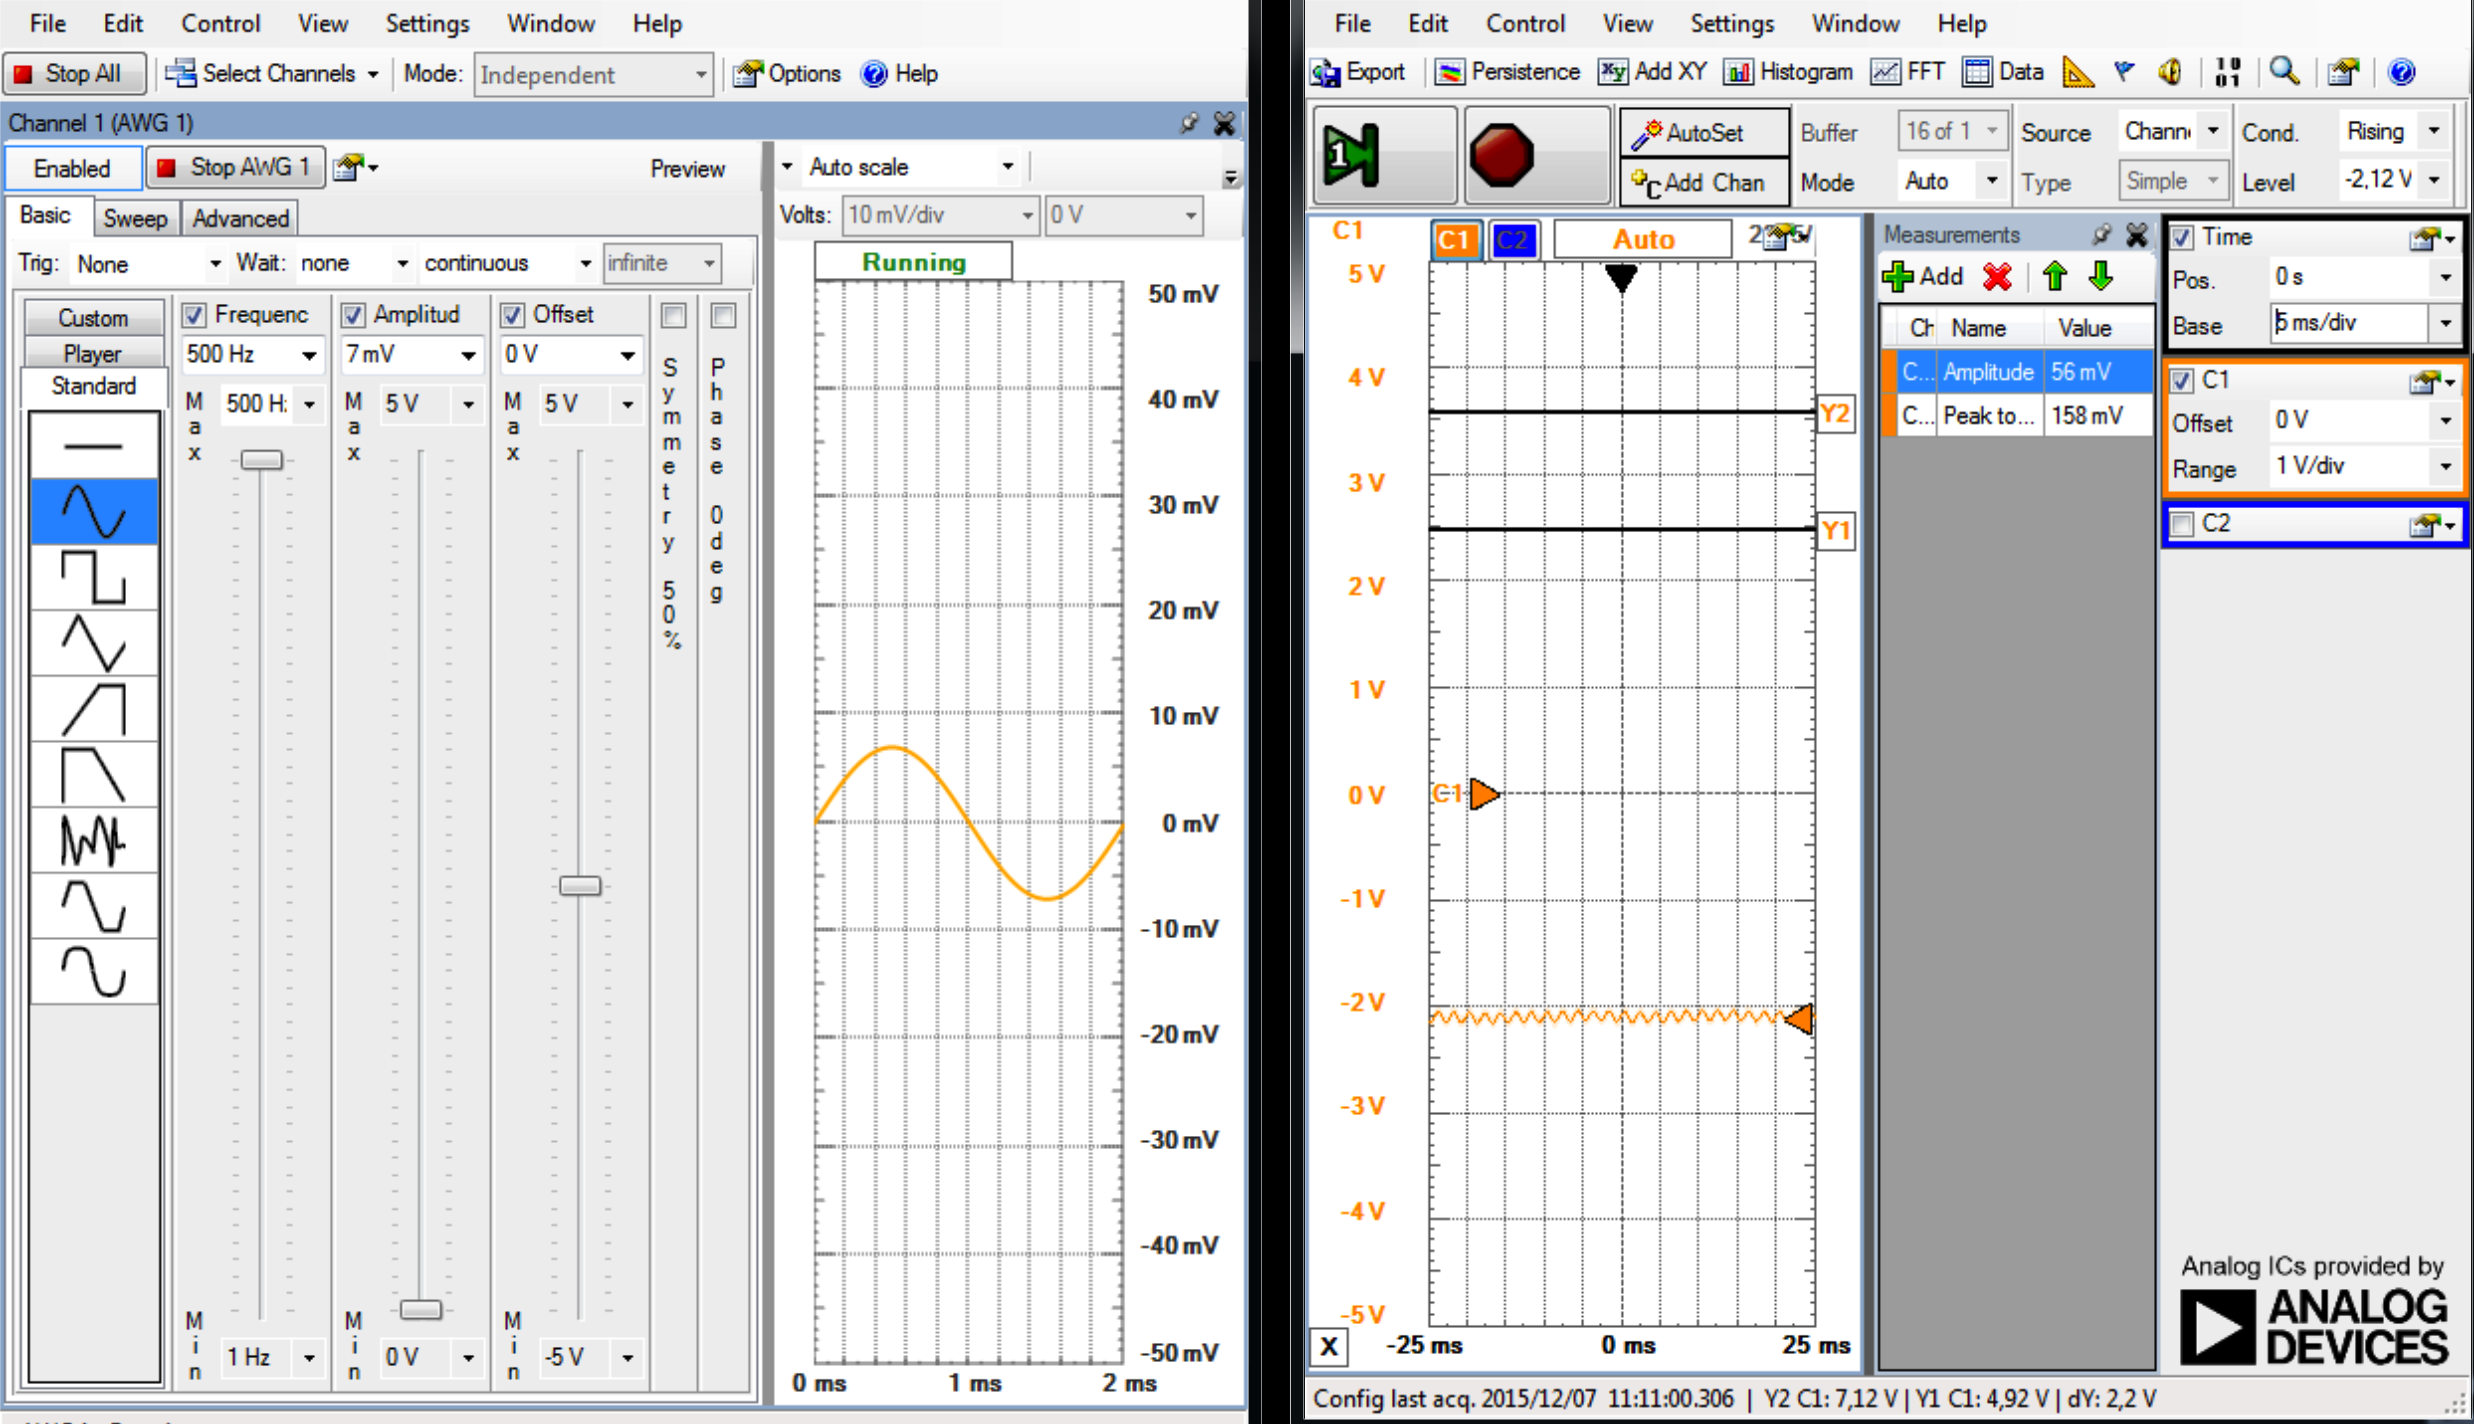
\includegraphics[width=1\textwidth]{Figurer/Snip20151207_45}
	\caption{Signalbehanlding respons 500 Hz}
	\label{fig:Signalbehanlding}
\end{figure}




